\documentclass{article}
\IfFileExists{microtype.sty}{\usepackage[final]{microtype}}{}
\IfFileExists{xurl.sty}{\usepackage{xurl}}{}
\usepackage[margin=1in]{geometry}
\usepackage{booktabs}
\usepackage{graphicx}
\usepackage{url}
\usepackage{hyperref}
\usepackage{amsmath}
\usepackage{enumitem}
\IfFileExists{xr-hyper.sty}{%
  \usepackage{xr-hyper}%
  \IfFileExists{supplement.aux}{\externaldocument[][nocite]{supplement}}{}%
}{%
  \IfFileExists{xr.sty}{%
    \usepackage{xr}%
    \IfFileExists{supplement.aux}{\externaldocument{supplement}}{}%
  }{}%
}
\setlength{\emergencystretch}{5em}
\hbadness=10000
\hypersetup{
  pdftitle={SPOT-OD: Adaptive-Filter and Observability Mechanism Findings from a Simulator-Bound Orbit-Determination Audit},
  pdfauthor={Authors omitted for review},
  pdfsubject={Orbit determination audit with adaptive filtering, observability diagnostics, sparse visibility, and evidence-boundary evaluation},
  pdfkeywords={orbit determination, adaptive filtering, observability diagnostics, sparse visibility, evidence audit, reproducibility, satellite state estimation, learned filtering, negative results}
}

\title{SPOT-OD: Adaptive-Filter and Observability Mechanism Findings from a Simulator-Bound Orbit-Determination Audit}
\author{Authors omitted for review}
\date{June 2026}

\begin{document}
\maketitle

\begin{abstract}
\noindent SPOT-OD studies a practical screening question for sparse-visibility orbit determination: when does adaptive measurement-noise tuning respond to dynamics mismatch by suppressing useful state corrections? In a fixed compact two-body+$J_2$+drag simulator, we compare tuned EKF, UKF, AUKF, offline batch WLS, structural-channel filters, and bounded learned residual estimators under common observed-step scoring.

The primary contribution is an OD-specific diagnostic of AUKF \(R\)-inflation under force-model mismatch. On the primary compact slice, AUKF raises the mean effective measurement-scale factor to 3.32 and its median \(R\)-only NIS to 4.73, compared with 1.60 for EKF and 1.83 for UKF, while damping the corrections needed to follow the biased dynamics. A drag-scale cascade then separates three mechanisms that can bind learned or adaptive candidates: EKF linearisation error, sparse-geometry observability, and candidate ballistic-coefficient inertia. A prospective sampled pre-update diagnostic over 10 synthetic scenario cells (80 realization rows, 960 trajectories, 22,574 observed steps) recomputes true pre-update \(R\)-only innovation ratios inside the UKF/AUKF recursions. At \(\rho_{\mathrm{pre}}\geq1.25\), the warning is highly specific but sparse: precision is 8/8 for AUKF-worse-than-best-nonadaptive (Wilson 95\% CI [0.68, 1.00]) with 8/52 recall (CI [0.08, 0.28]), while precision/recall against fixed-noise UKF are 6/8 (CI [0.41, 0.93]) and 6/37 (CI [0.08, 0.31]). A 16-row higher-fidelity pre-update rerun (192 trajectories, 4,482 observed steps) produces no warning firings at thresholds 1.10--1.50 despite AUKF-worse labels on 7/16 rows versus UKF and 10/16 versus the best nonadaptive filter. Together with a 3-hour higher-fidelity row that reverses the EKF/AUKF ordering, this confines the diagnostic to a compact-regime warning rather than a transfer rule.

The learned-estimator record is secondary. Internal frozen-rule replications of the originally audited residual/GNN/KalmanNet-style frozen endpoint family find no construction that beats the best tuned classical reference on observed-step position RMSE. A later retained-candidate learned-output branch is the first material learned-method PoC in the current package. In the new edge-only graph-path ablation, the attention residual-refinement ensemble improves retained non-development RMSE from 459.591~m to 373.728~m (18.682\%) and fresh unseen source-generation seed RMSE from 445.943~m to 364.229~m (18.324\%). Omitting node-disagreement aggregates reduces node features from 30 to 22 while preserving 10 pairwise edge features for graph-message-passing layers. The edge-only attention model cleanly beats the matched no-message local control (33.504\% all non-development and 55.270\% fresh aggregate advantage), while attention-vs-mean graph evidence is weaker/mixed. The earlier node-aggregate attention residual-refine result remains positive versus best retained (17.302\% and 16.035\%) but its graph-over-local intervals cross zero. These are retained-candidate compact-simulator results only, not standalone learned recursive filtering, operational validation, public precise-reference validation, broad learned-OD validation, or operational learned OD. A learned row-weighted DLS graph proof of concept beats fixed DLS on five credible-dense split seeds, but the gain is below the 3\% practical floor and a no-message control is nearly identical, so it is recorded only as a post-freeze compact-simulator side branch rather than public precise-reference validation, learned-superiority validation, or message-passing isolation. Public LAGEOS CRD/SP3 probes likewise remain support-only: the 260606 readout is indeterminate (learned-minus-best-classical $-6.66$~m, 95\% CI $[-205.84,+144.45]$~m), EDC has usable 260613 SP3 products, 260620 and 260627 remain unavailable/placeholder in the latest probes, and CDDIS remains login/HTML rather than parseable SP3.

Read as a compact-simulator mechanism-audit technical note, the materials provide a compact OD mechanism diagnostic and an inspection/reproducibility scaffold for deciding which estimator ideas merit higher-fidelity or real-data validation. It is not operational POD validation, not a reusable learned-OD framework, and not a general negative result for learned orbit determination.

\end{abstract}

\noindent\textbf{Keywords:} orbit determination; adaptive filtering; observability diagnostics; sparse visibility; evidence audit; reproducibility; satellite state estimation; learned filtering; negative results

\begin{table}[t]
  \centering\scriptsize
  \caption{Main-text abbreviation guide for the estimator and audit terms used in the Results.}
  \label{tab:main_abbreviation_glossary}
  \begingroup\setlength{\tabcolsep}{4pt}
  \begin{tabular}{@{}lp{0.34\linewidth}lp{0.34\linewidth}@{}}
    \toprule
    Term & Meaning & Term & Meaning \\
    \midrule
    OD/POD & orbit determination / precise orbit determination & EKF/UKF/AUKF & extended, unscented, and adaptive UKF filters \\
    PUKF & predeclared process-noise adaptive UKF & DMC-EKF & dynamic-model compensation EKF with empirical acceleration \\
    DSA-EKF/UKF & drag-scale adaptive EKF/UKF & RGR-GF & residual graph recurrent estimator with graph filtering priors \\
    DBAR & dynamics-bias adaptation-risk heuristic & NIS/CRLB & normalized innovation squared / Cramer-Rao lower bound \\
    SGP4/TLE & public-catalog propagator / two-line element set & SLR/SP3 & satellite laser ranging / precise-orbit state product \\
    CRD/ILRS & Consolidated Laser Ranging Data / International Laser Ranging Service & CDDIS & NASA/CDDIS SLR data archive \\
    WLS & weighted least-squares offline batch OD reference & RFIS/VG-RFIS & offline smoother and visibility-gated composite; see supplement glossary \\
    IDP-RGR-GF & identity-prior residual variant; see supplement glossary & Scope-only & retained for scope, stress, or provenance interpretation; not used for pass/fail conclusions or headline claims \\
    V\&V & verification and validation; used here as adjacent credibility lineage &  &  \\
    \bottomrule
  \end{tabular}
  \endgroup
\end{table}

\section{Introduction}

\paragraph{Contribution in one sentence.}
SPOT-OD turns the known adaptive covariance-matching failure mode into a sparse-OD screening diagnostic: AUKF \(R\)-inflation under force mismatch, a drag-scale cascade that localizes binding constraints, and an evidence audit that keeps learned-estimator positives from being promoted before higher-fidelity validation.

Satellite OD is grounded in orbital dynamics, measurement modelling, and recursive statistical estimation \cite{hoots1980spacetrack,vallado2006sgp4,vallado2013,montenbruck2000,tapley2004statistical}, with Kalman-filter families and their nonlinear extensions central because they encode physical priors, uncertainty propagation, and measurement-update structure \cite{kalman1960,jazwinski1970stochastic,julier1997unscented,wan2000unscented}. Sparse visibility --- intermittent contact, unfavourable geometry, and shifting noise statistics --- motivates adaptive filters and learned residual components, but it also raises the evidentiary bar for any claim that a learned estimator improves on a strong dynamics-aware baseline, which is the evidence boundary used here.

\paragraph{Scope and claim boundary.}
This is a compact-simulator mechanism-audit technical note. Its supported headline is the AUKF \(R\)-inflation and drag-observability diagnostic in the reported sparse-visibility simulator, with observed-step position RMSE as the primary endpoint; all-step trajectory RMSE is retained only as a propagation-dominated reference because roughly four-fifths of evaluated steps have zero visible stations. The study is not operational POD validation, not a reusable framework paper, and not broad learned-OD validation; public CRD/SP3 material is support-only measurement-pipeline and transfer-boundary evidence. Evidence was internally fixed before the claimed runs rather than externally registered, and conclusions are bounded to the tested constructions and sparse-visibility regimes. The secondary learned negative weighs against advancing the originally audited residual/GNN/KalmanNet-style constructions under this compact prior, geometry, and candidate set; it does not transfer as a claim about learned OD under a different force model, sensor suite, or public-reference regime. A later retained-candidate learned-output branch is the first material learned-method PoC in the current evidence package: the edge-only attention graph residual-refinement ensemble records 18.682\% all-nondevelopment and 18.324\% fresh gains versus the best retained candidate and supersedes the released pure selector. Its clean graph-path isolation is only versus the matched edge-only no-message local control; attention-vs-mean graph evidence is weaker/mixed, and the older node-aggregate graph-over-local residual intervals cross zero. The result is bounded as retained-candidate compact-simulator evidence rather than operational validation, operational learned OD, or a replacement for the original learned-negative endpoint. For exclusions and limitations, see Table~\ref{tab:main_claim_evidence_limit} and Section~7.

\paragraph{Evidence navigation aid.}
Table~\ref{tab:main_claim_evidence_limit} is the compact claim map. It separates the one load-bearing mechanism tier from secondary internal frozen-rule checks, support-only public CRD/SP3 probes, reproduction/inspection material, and exclusions/future validation tiers, so scored or pending public probes and post-freeze PoCs are not mistaken for operational validation.

\paragraph{Contributions.}
\emph{(C1) Adaptive-filter and observability diagnostic}: under force-model mismatch in a compact two-body+$J_2$+drag OD simulator, AUKF inflates effective \(R\) (mean 3.32; median \(R\)-only NIS 4.73 versus 1.60/1.83 for EKF/UKF) and damps state corrections. The drag-scale cascade separates EKF linearisation failure, sparse-geometry observability limits, and candidate-side \(\beta\)-prior inertia as distinct binding constraints, showing median trajectory-mean $\hat{\beta}=1.0000$ despite 9.6~km median arc-mean drag separation at enriched geometry. A prospective sampled pre-update cross-scenario campaign then bounds the diagnostic: at \(\rho_{\mathrm{pre}}\geq1.25\), high ratios have 8/8 precision for AUKF worse than the best nonadaptive EKF/UKF reference (Wilson 95\% CI [0.68, 1.00]) but only 8/52 recall (CI [0.08, 0.28]); against UKF alone, precision is 6/8 (CI [0.41, 0.93]) and recall is 6/37 (CI [0.08, 0.31]). A higher-fidelity pre-update repeat over J2..J4 and J2..J6 truth cells records zero warning positives at thresholds 1.10--1.50 while AUKF is worse than UKF on 7/16 rows and worse than the best nonadaptive reference on 10/16, so the warning is high-specificity/low-recall inside the compact sampled frame and non-transferable in this higher-fidelity repeat. A secondary mechanism finding is the long-arc EKF/AUKF ordering reversal: on 3-hour higher-fidelity arcs, AUKF has lower RMSE than EKF on the tested long-arc slice (EKF$-$AUKF mean $+264.4$~m, CI strictly above zero), showing that compact-model AUKF prescription is regime-bound.

\emph{(C2) Evidence-boundary and reproducibility scaffold}: the supporting record ties trajectory-unit paired resampling, practical-significance floors, visibility masks, structural-channel withdrawal rules, manifest checks, and bounded reruns to the paper's claim hierarchy. It is an inspection record within self-authored definitions, not evidence of transfer beyond this study.

\emph{(C3) Exploratory learned-estimator audit} (secondary): under the primary observed-step endpoint, the originally audited residual/GNN/KalmanNet-style learned family does not beat the per-scenario best tuned classical reference in the $K=32$ frozen-rule replication, and the PUKF/DMC-EKF/DSA-EKF variants and DBAR heuristic likewise miss their predeclared criteria. Because the endpoint was chosen after the training-cohort review and the $K=32$/$K=96$ checks are internal frozen-rule replications rather than external preregistration, this remains bounded screening evidence. A post-freeze retained-candidate learned-output branch now records a material learned-method PoC: the edge-only attention graph residual-refinement ensemble gains 18.682\% on all non-development rows and 18.324\% on fresh unseen source-generation seeds 151/157/163/167 versus the best retained candidate, with positive bootstrap intervals on both aggregates. It outputs a probability-weighted retained-candidate trajectory plus learned constant 3D per-candidate offsets, omits node-disagreement aggregates (22 node features rather than 30), preserves 10 edge features for graph-message-passing layers, and supersedes the released pure attention selector (13.691\% and 13.182\% gains versus best). The matched edge-only no-message local control is much weaker in aggregate (562.030~m all non-development and 814.283~m fresh), giving a positive graph-path/message-passing isolation result against that local control; the edge-only mean graph remains closer (386.224~m and 380.065~m), so attention-vs-mean evidence is weaker/mixed. The earlier node-aggregate attention residual-refine run remains positive versus best retained (380.074~m all non-development and 374.438~m fresh), but its graph-over-local residual intervals cross zero. This branch is not a standalone learned recursive filter, not operational evidence, not broad learned-OD validation, and not an erasure of the original learned-negative claim for the originally audited family. Post-freeze GraphAnchorPairGate, AdaptiveCandidateFusion, and row-weighted DLS probes remain compact-simulator side branches below confirmatory learned-superiority evidence; the row-weighted DLS graph beats fixed DLS on five credible-dense split seeds by only 0.054797~m mean fixed-minus-learned RMSE delta, remains below the 3\% practical floor, and is nearly matched by the no-message control.

\paragraph{Aerospace relevance.}
Sparse OD evidence is a campaign-design problem as much as an estimator-ranking problem. Aerospace OD claims depend on geometry, dynamics fidelity, and operational context, so the appropriate posture here is a bounded mechanism-audit note rather than a reusable validation framework. Recent studies span operational and public-data OD contexts \cite{ceresoli2025robust,oliveira2026opticalflow,liu2026epsa,lowe2026drag,lim2026publicorbitmaneuver}, alongside learned and adaptive filter applications \cite{zhang2026hnn}; SPOT-OD addresses compact adaptive-filter mechanism diagnosis and learned-estimator evaluation rather than operational public-orbit maneuver reconstruction. A practitioner takeaway: before committing to a precise-reference reduction or operations-facing validation campaign, an estimator-selection gate can require learned candidates to survive tuned adaptive guardrails, frozen endpoints, practical-significance floors, and provenance checks on a compact simulator. Learned estimators that fail these checks under compact dynamics remain pre-campaign hypotheses rather than validated upgrades; those that pass become candidates for higher-fidelity follow-up. SPOT-OD provides the compact-simulator gate mechanics: apparent positives are supported, bounded, demoted, or withdrawn by predeclared rules rather than post-hoc narrative.

\paragraph{Estimator family evaluated under the worked evidence package.}
The record covers tuned EKF/UKF/AUKF baselines, an offline robust batch WLS OD reference, the authors' bounded residual learners, a validation-tuned in-house KalmanNet-style learned-gain comparator (S-Table~\ref{tab:kalmannet_gain_inhouse_comparator}), and three predeclared dynamics-bias responses: PUKF, DMC-EKF, and DSA-EKF. The bounded learned-negative is not solely based on author-defined RGR residual variants: it also includes the in-house learned-gain comparator, a single canonical untuned Ensemble Kalman Filter (EnKF) comparator, and a narrow validation-only EnKF inflation audit that selected inflation \(1.00\), i.e., no added inflation, after larger inflation values degraded validation performance. Localized EnKF, particle-filter, Gaussian-mixture, ensemble-size-search, and broader EnKF hyperparameter variants remain outside the tested scope. Post-freeze GraphAnchorPairGate, AdaptiveCandidateFusion, trajectory candidate selector, and row-weighted DLS probes use different estimands, anchors, or retained-candidate routing and are documented as compact-simulator PoCs rather than treated as part of the originally audited residual/GNN/KalmanNet-style observed-step family. The main text keeps the learned side to summary boundary evidence; detailed learned-comparator diagnostics (including the $K=96$ stress replication, EnKF checks, structural-channel checks, and post-freeze portfolio probes) are housed in the supplement so the central C1 mechanism finding remains visible.

\paragraph{What survives scrutiny.}
Reviewers can verify the compact AUKF \(R\)-inflation mechanism (Table~\ref{tab:main_aukf_mechanism}, Figure~\ref{fig:aukf_r_inflation_mechanism}), the drag-scale cascade, the secondary learned-negative across $K=32$/$K=96$ internal frozen-rule replications, DBAR withdrawal plus support-only public CRD/SP3 readouts, and the inspection record tying seeds, rules, evaluations, digests, and validation artifacts to claims. Table~\ref{tab:main_claim_evidence_limit} states the governing scope boundaries; bounded reruns and live public-week scoring remain inspection material below full independent scientific reproduction.

\paragraph{Bounded negative outputs.}
The secondary negatives are bounded to the tested constructions. No originally audited residual/GNN/KalmanNet-style learned construction beats classical on $K=32$ observed-step; $K=96$ stress preserves that negative at floor-power scale. DMC-EKF is not better than UKF (CI $[-3.8,+8.1]$~m), DSA-EKF is below its practical floor and remains worse than AUKF on the 3-hour long-arc replication (CI $[+8.7,+697.9]$~m), and DBAR is withdrawn after its 450-realization characterization is statistically indistinguishable from an $81.3\%$ no-information baseline. Later GraphAnchorPairGate, AdaptiveCandidateFusion, retained-candidate learned-output/selector, and row-weighted DLS probes are supplement/archive or compact main-text PoC diagnostics, not counterfactual reruns of the frozen observed-step endpoint. The edge-only attention graph residual-refinement ensemble is positive and strongest within the current retained-candidate learned-output branch; within that edge-only setup it isolates a graph-path advantage over the matched no-message local control, but attention-vs-mean is weaker/mixed and the branch still depends on retained candidates and simulator truth-supervised training. It therefore does not become a standalone learned recursive filter or operational learned OD validation. Row-weighted DLS improves fixed DLS by about 0.05~m and raw EKF/UKF by about 0.58\% on the credible-dense slice, below the 3\% practical floor and without isolating message passing. See Table~\ref{tab:main_claim_evidence_limit} and supplement S-tables for scope.

\paragraph{Measurement-geometry observability diagnostic cascade on the drag-scale structural channel.}
A three-slice \emph{measurement-geometry observability diagnostic cascade} on the augmented multiplicative drag-scale parameter $\beta$ is reported in the Results after the structural-channel estimators and decision predicate have been introduced, with full details in the supplement (supplementary Sections~\ref{app:constructive-positive-control}--\ref{app:observability-positive-control-ukf}). Each slice fixes the drag-scale channel as the structural form matched to the synthetic bias, freezes the candidate hyperparameters from the prior validation selection, and applies the predeclared structural-channel decision predicate unchanged; all three slices return predeclared bounded structural-channel negatives. The cascade is reported as a mechanism diagnosis, not as a calibration positive for the evidence package.

\section{Related Work and Positioning}
\paragraph{Orbit propagation and statistical estimation.}
The study is grounded in the SGP4/NORAD lineage and standard astrodynamics references \cite{hoots1980spacetrack,vallado2006sgp4,vallado2013,montenbruck2000}, with statistical OD providing the framework for combining dynamics, measurements, and uncertainty \cite{tapley2004statistical}. This motivates a baseline-first stance: learned methods must be evaluated against strong physical filters, not weak comparators.

\paragraph{Recursive filters and learned filtering.}
The Kalman filter \cite{kalman1960}, EKF \cite{jazwinski1970stochastic} and the unscented transform \cite{julier1997unscented,wan2000unscented} are standard recursive estimators. Adaptive Kalman methods motivate innovation/smoother-based noise adjustment; learned filtering, including KalmanNet, motivates hybrid designs \cite{mehra1970adaptive,kruse2025adaptive,haarnoja2016,revach2022kalmannet,mortada2025recursivekalmannet}. An independent physics-informed ML cislunar OD study reinforces that learned-OD evaluation must weigh calibration and uncertainty rather than point accuracy alone~\cite{badura2025piml}; deep-neural nonlinearity detectors driving order-switching filters are complementary neural-aided designs~\cite{zhou2023orderswitching}. Improvements over fixed-noise UKF can reflect noise-adaptation already represented by AUKF. Classical adaptive filtering recovers noise statistics only when the model structure is correct \cite{mehra1970adaptive,sage1969adaptive,jazwinski1970stochastic}; robust Kalman work on heavy-tailed noise is adjacent context, not a direct OD baseline \cite{wang2026heavytailedkf}. The AUKF result reported here instantiates the known covariance-matching limitation under model mismatch established in the classical adaptive-filter literature: when the dominant residual is dynamics or force-model error rather than noise-distribution error, adaptive noise-statistics adjustment can degrade rather than improve estimation \cite{mehra1970adaptive,sage1969adaptive,jazwinski1970stochastic}. The OD-specific quantification here is that AUKF inflates effective $R$ under compact-model force-bias in sparse-visibility OD. Chihabi \& Ulrich (2025) provide recent angle-only adaptive OD context, confirming that learned and adaptive filter performance depends on the source of residual mismatch (dynamics-side bias versus noise-side distributional error) \cite{chihabi2025adaptive}. When the dominant residual is dynamics/force-model error, statistical OD prescribes \emph{dynamic model compensation} (DMC): state augmentation with low-frequency empirical-acceleration estimates to absorb unmodelled accelerations through process-model channels rather than noise reweighting \cite{tapley2004statistical,wright1981drag,stacey2021adaptive,wang2026empiricalacceleration}. The force-mismatch and structural-channel results reported below are controlled diagnostics consistent with this lineage.

Recent learned and adaptive OD studies (2023--2026) cover: systematic LEO precise-OD reviews~\cite{selvan2023precise}; physics-informed neural OD, optical IOD/tracklet-correlation, and learned/adaptive filters across ground-based, SSA, cislunar, deep-space, relative-navigation, and continuous-maneuver regimes~\cite{scorsoglio2023pinn,scorsoglio2026xgeo,ramponi2026pontryagin,zhou2023lstm,zhang2024libration,pinheiro2024flexkalmannet,gao2025heavytailed,sztamfater2026sequential,xu2026arckf,li2026delay,zhang2026hnn,chen2024robust,zhu2025bayesian}; operational orbit-recovery, drag-estimation, TLE refinement, hybrid SGP4 error-learning, and continuous-maneuver OD~\cite{chen2026orbitrecovery,lowe2026drag,belyakov2025satellites,segura2026hybridsgp4,liu2026lowthrustpiecewise}; cislunar IOD, optical-flow IOD, ISL observability, multi-scale initializers, and TLE global-optimization~\cite{smego2026dynamic,heidrich2025collocation,ojedaromero2025adaptivecislunariod,song2026multiconstrainediod,oliveira2026opticalflow,li2026islheterogeneous,zhu2026multiscale,liu2026epsa}; and cislunar PGM/hybrid filtering, orbit-attitude/sensor-tasking coupling, and real-spaceborne GNSS adaptive EKF~\cite{paranjape2026probabilistic,paranjape2026hybridpgm,paul2026mukf_tasking,cossu2026lugre,lang2025starlinkunscented}. Recent 2026 learned-orbit predictors~\cite{liao2026patchtransformer,yang2026lstmtransformerorbit,mahmud2026pinnleo} address propagation/orbital-parameter forecasting rather than recursive state-estimation evidence-boundary audits under fixed force models and sparse visibility. These complementary studies report estimator performance in their own regimes; SPOT-OD asks what evidence composition screens learned or adaptive improvement claims. SPOT-OD does not propose a new estimator; it places learned residual methods, noise-adaptive AUKF/PUKF, structural DMC-EKF, public replay, and selector tasks under one auditable evidence boundary. Domain-adjacent neural orbit/state-estimation and spacecraft-GNN work \cite{varey2024physics,kiprit2026temporalgrid} shows learned satellite inference is not new, without making those papers direct baselines here.

\paragraph{Worked evidence package.}\label{sec:novelty-audit}\label{sec:protocol-prescription}
The seven ingredients (predeclaration, paired bootstrap, Holm/BH multiplicity control, capacity-matched controls, upstream architecture sanity reproduction, astrodynamics-grounded floors, evidence-record traceability) are individually standard practice in adjacent literatures~\cite{morris2019simulation,bouthillier2021accounting,dehghani2021benchmark,pineau2021reproducibility,semmelrock2025reproducibility,min2026transparency,ode2026protocol,yeo2020nistir}. Here they make the retained evidence inspectable for the compact AUKF and drag-scale mechanism claims; because the definitions are author-defined, they are a boundary rather than an independent source of novelty evidence. The supplement provides a scoped visible-record positioning audit as an inspection aid (S-Table~\ref{tab:novelty_audit_systematic}, supplementary Section~\ref{app:novelty-audit-systematic}), not an absence proof, independent novelty proof, or validation. S-Table~\ref{tab:protocol_subset_ablation} is a subset-sufficiency audit showing, ingredient by ingredient, that omitting a named ingredient would have admitted a misleading positive or unsupported upgrade in this evidence set. The result is a worked evidence package for this compact sparse-visibility study, not demonstrated cross-domain transfer. Reuse in GNSS-LEO, optical, SLR, or operations-facing OD would require rebuilding the ingredients around that domain's measurements, force model, reference products, baselines, and predeclared gates, followed by independent application by a party other than the record designer.

\begin{table}[t]
  \centering\scriptsize
  \caption{Compact claim--evidence map for this technical note. The rows separate the load-bearing compact mechanism evidence from secondary internal checks, support-only public probes, reproduction/inspection material, and excluded future validation tiers.}
  \label{tab:main_claim_evidence_limit}
  \begingroup\setlength{\tabcolsep}{3pt}
  \begin{tabular}{@{}p{0.14\linewidth}p{0.20\linewidth}p{0.34\linewidth}p{0.24\linewidth}@{}}
    \toprule
    Tier & Load-bearing status & Evidence & What it cannot establish / next tier \\
    \midrule
    1. Primary compact mechanism & Load-bearing mechanism evidence & AUKF effective-$R$ inflation under compact force-model mismatch plus the drag-scale cascade separating EKF linearisation, sparse-geometry observability, and candidate inertia (Table~\ref{tab:main_aukf_mechanism}, Figure~\ref{fig:aukf_r_inflation_mechanism}, Table~\ref{tab:main_drag_scale_cascade}). & Cannot establish operational POD, a reusable framework, or a transferable EKF/AUKF prescription; next tier is precise-reference or higher-fidelity validation. \\
    2. Secondary learned-negative & Internal frozen-rule evidence; not external preregistration & No evaluated learned construction beats the per-scenario best tuned classical reference on the selected observed-step endpoint across $K=32$/$K=96$ internal replications. & Cannot rule out all learned OD systems or confirm the endpoint externally; next tier is prospective external confirmation on an independently fixed protocol. \\
    3. Public CRD/SP3 probes & Support/provenance only & Public LAGEOS CRD/SP3 readouts exercise parsing, reduction, state scoring, traceability, breadth, and DBAR/calibrator boundaries; scored public-week readouts and pending/unscored rules are separated from validation claims. & Cannot validate the compact simulator conclusion, centimetre SLR, operational POD, or real-data learned-estimator skill; next tier is independently predeclared public-reference scoring. \\
    4. Reproduction and inspection & Access/integrity tier satisfied; scientific rerun still bounded & Public DOI/GitHub archive deposition, manifests, digests, archive extraction, active manuscript artifact regeneration, one archived-input public OD slice rerun, one bounded learned-estimator replay, and one non-destructive full rerun are retained with a divergence audit. & Cannot establish clean full scientific reproduction, independent-machine reproduction, full raw/training/all-filter public reproduction, live public-data retrieval, operational POD, third-party independent validation, or replacement manuscript metrics. \\
    5. Exclusions and future validation & Not claimed; next evidentiary tiers & Operational POD, independent-machine reproduction, full raw/training/all-filter reruns, broader learned OD, localized EnKF, particle/Gaussian-mixture filters, and broader EnKF hyperparameter searches remain outside the current claim. & These exclusions cannot be inferred as deferred positives; they require new archived, independently rerun, or externally validated studies. \\
    \bottomrule
  \end{tabular}
  \endgroup
\end{table}

\paragraph{Positioning vs operational POD/SLR practice and recent learned satellite estimators.}
Operational precise OD on satellite-laser-ranging targets routinely reaches few-centimetre orbit accuracy at international analysis centres, with a full force model, a strict ITRF$\leftrightarrow$GCRF reduction ingesting the IERS Earth-orientation series, precise tropospheric and centre-of-mass corrections, and dedicated ranging campaigns coordinated through the ILRS \cite{pearlman2002ilrs,ilrs_npt_data,cddis_slr_npt,ilrs_crd_format}. Recent operational SLR/POD studies further demonstrate that precision depends on fusion strategy, range-bias handling, and prior constraints \cite{ren2026slrbds3,lemoine2026std2400}. The public precise-reference probes here share inputs and reference products with that practice but evaluate \emph{compact}-dynamics estimators (two-body+$J_2$, optional drag/third-body/SRP) under sparse-visibility recursive filtering; the resulting tens to hundreds of metres magnitudes are \emph{not} an operational precise-OD result and are not comparable to centimetre-class ILRS analyses. Their constructive role is narrower: they reduce measurement parsing, frame-reduction, state-scoring, and provenance risk before any later public-reference validation study. SPOT-OD does not propose a new estimator but reports a disciplined, predeclared negative on the authors' own residual constructions, leaving the comparison against any faithfully reproduced published learned-OD system explicitly open.

\paragraph{Graph neural networks, calibration, and observability.}
GNNs encode relational inductive biases through message passing \cite{kipf2017,hamilton2017,velickovic2018,battaglia2018relational,gilmer2017neural,scarselli2009graph}; the SPOT-OD ablation evaluates message passing variants under capacity and input matched controls but does not isolate them as the unique source of improvement (Section~\ref{sec:claim-audit}; \emph{graph message passing is not a claimed contribution} canonically there). Adjacent SSA work has also framed large-scale resident-space-object conjunction screening as a GNN link-prediction/screening problem, which is useful context but not a direct OD estimator baseline here \cite{chu2026conjunctiongnn}. Calibration analysis \cite{guo2017calibration} is used only as a diagnostic for the evaluated runs, not a deployment guarantee. Sparse OD is also an information problem; classical OD treats geometry and conditioning as central \cite{tapley2004statistical}, and prior space object observability work motivates explicit geometry analysis \cite{friedman2018space}. The finite difference geometry summaries are not a formal observability proof.

\section{Data Sources, Evaluation Scope, and Protocol}
\subsection{Archived data sources and scenario scope}
The public-data layer uses archived CelesTrak and SatNOGS snapshots rather than live API state. CelesTrak general-perturbation/TLE data provide public orbital element evidence \cite{celestrak_gp}; SatNOGS network, observation, and API metadata provide public ground-station and observation context \cite{satnogs_network,satnogs_observations,satnogs_api}. The retained records identify source URLs, fetch timing, record counts, and digests so replay scenarios remain fixed. Primary accuracy tables use the nominal and stress synthetic splits. Public-catalog SGP4 replay is a \emph{bounded public-catalog replay/reference slice} rather than a discriminative leaderboard: only the offline robust batch WLS reference produces a meaningful postfit solution. A controlled force-model/process-noise mismatch split inflates the truth drag/SRP/process-noise force model while estimators keep the nominal compact model. Bounded public precise-reference probes score real ILRS satellite-laser-ranging normal points for LAGEOS-1 and LAGEOS-2 \cite{pearlman2002ilrs,ilrs_npt_data}, parsed from public daily CRD version-2 files \cite{ilrs_crd_format} archived by the ILRS/NASA CDDIS data centers \cite{cddis_slr_npt}. None of these slices is operational flight validation.

The public-data inventory and the per-scenario provenance digests are recorded in S-Table~\ref{tab:public_data_summary}.

\subsection{Evaluation tasks}
SPOT-OD is an evaluation suite. The evaluated tasks are state estimation (acceptance-critical) and method selection (an internal synthetic routing diagnostic; see S-Table~\ref{tab:benchmark_tasks}). Stability labels serve exclusively as computational guardrails for the engineering-failure audit defined below.

A trajectory is numerically divergent when its trajectory-level position RMSE is non-finite or exceeds \(10^8\) m, or its velocity RMSE exceeds \(10^5\) m/s; method-selection costs assign a \(10^8\) m penalty to divergent candidates. These are computational guardrails, not physical stability certificates, so the results add a separate engineering-failure audit at 100 km position RMSE or 100 m/s velocity RMSE.

\subsection{State, dynamics, and observations}
Each trajectory has a six-dimensional Earth-centered inertial state
\begin{equation}
  x_t = [r_x,r_y,r_z,v_x,v_y,v_z]_t,
\end{equation}
with position in meters and velocity in meters per second. The generator uses a fourth-order Runge--Kutta Cartesian ECI propagator with 20 s steps for 120 steps. Nominal sampling uses altitude 450--950 km, eccentricity 0--0.02, inclination 20--98 degrees. The acceleration model includes two-body gravity, \(J_2\), drag against a co-rotating exponential atmosphere, optional point-mass Sun/Moon third-body terms, and optional solar-radiation pressure with a cylindrical Earth-shadow test. The reported nominal/stress splits use ballistic coefficient 0.018 m\(^2\)/kg, \(\rho_0=4.0\times10^{-11}\) kg/m\(^3\), \(h_0=400\) km, \(H=60\) km, third-body and SRP enabled, area-to-mass 0.02 m\(^2\)/kg, \(C_R=1.35\), and zero truth process noise. The force model is intentionally compact rather than flight-dynamics complete: it omits high-order geopotential, precession/nutation, empirical atmosphere, maneuvers, and sensor-scheduling uncertainty beyond the specified perturbations.

The measurement model is a station--satellite line-of-sight observation \(z_{t,s}=[\rho,\alpha,\epsilon,\dot{\rho}]_{t,s}\) (range, azimuth, elevation, range-rate); a station is visible at elevation \(\geq 8\) degrees. The nominal configuration uses eight ground stations. Nominal measurement noise is range 30 m, azimuth/elevation 0.02 degrees, range-rate 0.08 m/s, outlier probability 0.01, outlier scale 6, dropout 0.02, with small station/clock bias. The reported stress-test override increases range noise to 70 m, azimuth/elevation noise to 0.06 degrees, range-rate noise to 0.22 m/s, outlier probability to 0.04, and outlier scale to 10. These are protocol facts, not inferred from result tables.

\subsection{Splits, seeds, and evaluation units}
The main experiment uses seed 42. The dataset contains 160 nominal training, 32 nominal validation, 64 nominal test trajectories, 96 stress-training, 24 stress-validation, and 64 stress-test trajectories. The curriculum uses nominal pretraining, mixed training, and stress fine-tuning; later validation includes a SatNOGS replay split. All methods are scored on steps 11--119 (109 evaluated steps); nominal and stress aggregates summarise $64\times109=6976$ evaluated trajectory-steps each. The paired statistical unit is the trajectory-wise position RMSE over the same 109-step window, so Wilcoxon comparisons use $n=64$ paired trajectory values per comparison. All filters and learned models receive the same simulated measurements, visibility masks, station geometry, and noisy initial state estimates (2500 m position, 6 m/s velocity standard deviation); learned residual methods additionally receive the relevant filter priors.

\section{Methods Compared}
Estimator abbreviations are defined at first use, with a compact main-text guide in Table~\ref{tab:main_abbreviation_glossary} and a longer glossary at the start of the supplement. The compared families are classical recursive filters (EKF, UKF, AUKF), predeclared adaptive or structural variants (PUKF, DMC-EKF, DSA-EKF), an offline robust batch WLS OD reference, the bounded RGR residual learners and controls, and KalmanNet-related sanity/transposition diagnostics.

\subsection{Classical filtering baselines}
The EKF \cite{jazwinski1970stochastic}, UKF, and AUKF estimate the same six-dimensional state from common range/azimuth/elevation/range-rate observations (UKF unscented-transform parameters $\alpha_{\mathrm{UT}}=0.2,\beta_{\mathrm{UT}}=2,\kappa_{\mathrm{UT}}=0$; AUKF adds innovation consistency $R$ adaptation: rate 0.08, measurement scale bounds 0.4--30, Huber 2.8, NIS soft gate 16). The unscented-transform beta parameter is denoted \texttt{beta\_UT} in prose and \(\beta_{\mathrm{UT}}\) in equations; it is distinct from the drag-scale beta. Classical hyperparameters were selected through a 48-trial tuning budget. We also include an offline \emph{robust batch weighted least squares OD reference}: per trajectory it fits one initial Cartesian state to the full visible arc using the same force/measurement model and a Huber robust objective. This is intentionally non-causal and postfit --- a classical OD reference that can use future measurements, not a deployment equivalent comparator. We additionally include a \emph{process noise adaptive UKF (PUKF)} as the symmetric counterpart of the AUKF: it holds $R$ fixed at the nominal vector and inflates the predicted process noise $Q$ multiplicatively when a sliding window estimate of the $R$-only normalized innovation squared exceeds the chi-square-with-4-channels expectation, on the classical statistical OD intuition that under a dynamics/force model bias the prior model, not the measurement channel, carries the misspecified component \cite{mehra1970adaptive,jazwinski1970stochastic,stacey2021adaptive}. The PUKF rule, thresholds, and decision predicate are fixed in a timestamped rule record.

Ensemble Kalman and sequential Monte Carlo OD/data-assimilation methods are a distinct comparator family rather than a small variant of the tuned EKF/UKF/AUKF guardrail used here; they introduce ensemble-size, stochastic process-parameter, resampling, and sampling-noise design choices, and recent OD work explicitly evaluates EnKF and particle-filter tracking/parameter-estimation variants in that family \cite{sztamfater2026sequential}. To close the ensemble-Gaussian-filter exclusion rather than only cite it, we add one \emph{canonical untuned stochastic perturbed-observation Ensemble Kalman Filter} (EnKF) \cite{evensen1994sequential,burgers1998analysis} as a bounded auxiliary comparator: a 64-member ensemble propagated through the same compact two-body, $J_2$, and exponential-drag dynamics and updated with the same range/azimuth/elevation/range-rate measurement, process-noise, and azimuth de-weighting model as the EKF/UKF/AUKF baselines, with inflation and localization deliberately left off and a per-trajectory seed fixed in an internally frozen, hash-recorded rule that is an internal pre-evaluation record, not an externally timestamped pre-registration. Because the EnKF shares its process-noise and initial-covariance settings with the UKF and AUKF, the controlled comparison is EnKF versus UKF/AUKF, while the EnKF-versus-EKF gap additionally reflects the EKF's slightly larger tuned process noise. On the force-mismatch, nominal, and stress slices the untuned EnKF does not displace the classical filters (S-Table~\ref{tab:enkf_comparator}); in the current rerun its mean observed-step RMSE is 501.5, 390.0, and 1391.0~m versus best non-EnKF means of 431.2~m (EKF), 376.4~m (EKF), and 837.3~m (AUKF), respectively, so the predeclared positive criterion is unmet in all three slices. A subsequent validation-only inflation audit (S-Table~\ref{tab:validation_tuned_enkf_comparator}) selected \(1.00\), i.e., no added inflation, because larger grid values worsened the weighted validation score; the frozen test readout likewise produced no EnKF positive. The EnKF evidence is therefore reported as bounded to the canonical configuration and this narrow inflation audit; localized EnKF, particle/Gaussian-mixture filters, ensemble-size search, and broader process-noise or covariance retuning remain outside this comparator set.

\subsection{Learned estimator architecture and inputs}
Station nodes contain the scaled four-channel measurement, a visibility indicator, Earth-radius-scaled station coordinates, and optional innovation features. Graph-enabled models apply message-passing layers over an implicit fully connected station graph; graph-disabled variants either skip those layers or replace them with equal-depth local per-station layers. Visible embeddings are pooled and passed through a bidirectional GRU over a 12-step window. The training uses hidden dim 192, five graph layers (when enabled), two GRU layers, dropout 0.10, batch 128, lr $10^{-3}$, weight decay $10^{-4}$, grad-clip 1.0, mixed precision, early-stop patience 10, and a 24/18/12-epoch nominal/mixed/stress curriculum. The full architecture and regularizer weights are in Appendix~\ref{app:architecture}; the supplementary evidence materials supplied for independent inspection provide the complete reproduction records.

\paragraph{Hyperparameter and selection transparency.}
All compared families expose their fixed settings either in this Methods section, the reproduction checklist, or the supplement: EKF/UKF/AUKF use the common state, dynamics, observation, and noise settings stated above with the UKF and AUKF parameters stated here; PUKF, DMC-EKF, and DSA-EKF use predeclared rule records and the Gauss--Markov hyperparameters listed in the reproduction checklist; prior-guided learned variants share the same inputs, backbone dimensions, curriculum, optimizer settings, bounded-residual scale, gate, context budget, and prior-anchoring penalty stated here and in Section~\ref{sec:methods-families}; and KalmanNet-related checks use their separately scoped native-benchmark, transposition, and validation-grid records. Selection fairness is enforced before held-out scoring: for each held-out slice the candidate family, validation grid, selected setting, primary metric, comparator set, practical floor, seed/split identifiers, and pass/fail rule are fixed before the test population is evaluated, and no method is retuned after seeing held-out outcomes. Validation-tuned choices are linked to validation records rather than test outcomes, and trained-model/evaluation records are included so that every displayed row can be inspected without inferring hidden hyperparameters from the result tables.

\subsection{Method families}\label{sec:methods-families}
\textbf{Classical filters} are EKF, UKF, AUKF, and the predeclared process noise adaptive UKF (PUKF). \textbf{The classical postfit OD reference} is robust batch WLS, reported separately because this \emph{postfit classical OD reference} is offline rather than causal.

\textbf{The published learned OD baseline} is the KalmanNet release~\cite{revach2022kalmannet}, exercised on its own linear canonical benchmark as the upstream architecture sanity reproduction (S-Table~\ref{tab:kalmannet_official_reproduction}). The in-house KalmanNet-style learned-gain comparator keeps the EKF prior and flow and replaces the analytic gain with a bounded learned gain correction driven by normalized innovations and shared features; its gain scale and correction clip are selected by held-out validation loss over a small predeclared grid with no test-set information. It is a load-bearing in-house boundary comparator, not an official KalmanNet reproduction or exhaustive design-space test; the documented KalmanNet transposition is retained separately as a feasibility/design-gap diagnostic, not architecture-level refutations or learned-claim evidence.

\textbf{Prior guided learned variants} (flagship RGR-GF plus No-Graph Residual, Learned Noise Adaptive, IDP-RGR-GF, OI-RGR-GF) share a common backbone: a bounded residual \(\hat{x}=\hat{x}_{\mathrm{prior}}+g\odot(b\,s\tanh(r_\theta))\) with $s=0.03$, $g\in(0,1)^6$, $b\in(0,1)$, plus a $0.05\,\lVert\hat{x}-\hat{x}_{\mathrm{prior}}\rVert^2$ prior anchoring penalty; the gate $g$ and budget $b$ form a per-component learned trust region around the fused prior, whose variance-minimising operating point collapses toward the prior on the majority of steps where the visible measurements expose little prior-unexplained residual, so any ``competitive with classical'' behaviour is in substantial part inherited from the classical prior bank by construction; the \textbf{EKF residual learner} is a learned residual control (not a KalmanNet reproduction), retained only as an ablation row to bound the EKF only residual variant; it diverges substantially from EKF on the all-step propagation reference (S-Table~\ref{tab:main_results}) and is excluded from the claim audit's pairwise comparisons because it does not share the bounded residual contract of the RGR-GF family. \textbf{Input matched message passing controls} are RGR-noMP (skip control bypassing cross station aggregation) and RGR-local (stricter capacity matched control replacing the graph stack with equal depth, equal width local per-station layers). The matched budget ablations share splits, training stages, hyperparameter budget, and evaluation window, not exactly equal parameter counts or inputs. An unconstrained \textbf{Pure GNN} state predictor (no filter prior) is retained only as a supplementary sanity-check row (S-Table~\ref{tab:pure_gnn_training_sanity}); it diverges by orders of magnitude on every slice and is not used in any audit comparison.

\textbf{Trajectory candidate selector/residual-refinement ensemble} is a post-freeze compact-simulator PoC rather than part of the original frozen endpoint family. It is learned routing over retained candidate trajectories from \texttt{EKF}, \texttt{UKF}, \texttt{AUKF}, \texttt{BatchWLS}, \texttt{RFIS}, and \texttt{VA\_RFIS}; it uses retained truth-free candidate, visibility, eval-mask, scenario, and configured candidate-disagreement features, while eval truth is used only to score rows and baselines. The released pure selector averages candidate probabilities arithmetically across selector seeds 2001, 2005, and 2009. The residual-refinement branch uses member seeds 2111, 2117, and 2129, averages candidate probabilities and constant 3D per-candidate offsets, and outputs a probability-weighted retained-candidate trajectory plus learned offsets. The new edge-only ablation sets \texttt{--node-disagreement-features omit}, reducing the node dimension from 30 to 22 while leaving the 10 pairwise edge distance/overlap features available only to graph-message-passing layers. These runs route/refine already generated candidates, not operational OD validation, not public precise-reference validation, not standalone learned recursive filters, and not broad learned-OD evidence; the graph-path isolation claim is limited to edge-only attention versus the matched no-message local control.

\textbf{Learned row-weighted damped least-squares correction} is a post-freeze compact-simulator PoC rather than part of the original frozen endpoint family. Around a validation-selected EKF anchor, DLS alpha, and damping value, a station graph-message-passing model predicts per-measurement-row weights inside the damped least-squares normal equations. The evaluated slice is \texttt{credible\_dense\_od\_test} with candidate methods \texttt{EKF,UKF}, DLS anchor \texttt{EKF}, alpha grid \(-0.2,-0.1,-0.05,0.05,0.1\), damping/lambda grid \(100,1000\), row-weight granularity, random weight-head initialization, weight regularization \(0\), log-weight-scale \(2.0\), full precision/no AMP, and split seeds 7, 11, 13, 17, and 19. Full precision is required and is now the default for this differentiable solve because AMP previously prevented parameter updates.

\subsection{Observability-geometry features and guarded selection}
Per step, SPOT-OD computes a local unweighted measurement-geometry Gramian from finite-difference Jacobians of the normalized measurement model with respect to scaled state, \(\mathcal{I}_t=\sum_{s\in\mathcal{V}_t}H_{t,s}^{\top}H_{t,s}\). The summary uses clipped log trace, log pseudo-determinant, log condition number, rank fraction, visible-station fraction, and minimum-eigenvalue features (causal: computed from the filter prior, not truth). The guarded selector is a separate trajectory-level cost predictor over visibility, public/stress flags, innovation energy, prior disagreement, and these summaries; it is an internal evaluation safeguard, not a proof of operational autonomy.

\subsection{Statistical protocol}\label{sec:statistical-protocol}
\paragraph{Endpoint terminology (defined once, used throughout).}
\emph{This study is exploratory}\footnote{In statistical methodology, \emph{exploratory} analysis selects endpoints or hypotheses after inspecting data patterns, while \emph{confirmatory} analysis tests pre-registered hypotheses on held-out data. This study's endpoint timeline is exploratory with internal frozen-rule replications ($K=32$ and $K=96$ draws), not externally pre-registered confirmatory validation.}: the commitments are internal predeclarations supplied with the submission, with timestamped records where the record format supports them, not external trial-registry preregistration or confirmatory validation. \emph{Predeclared} means a metric, threshold, or decision rule written down before the run that produced its result. The $K=16$ frozen-rule extension has a confidential RFC3161 timestamp of its rule hash (hash disclosed, not content); the timestamp confirms rule-before-evaluation ordering for that draw but is not public preregistration and does not upgrade the observed-step endpoint itself from post-hoc to externally predeclared. Evidentiary control comes from retained internal rule records, fixed seeds/splits, and digest-linked evaluation records, which make post-hoc rule substitution inspectable under internal frozen-rule consistency but do not provide confirmatory external validation.

\emph{Endpoint timeline (summarized; full details in supplement):} Observed-step RMSE was selected post hoc on the training cohort before $K=32$ generation. $K=8$ internal record froze the selected endpoint on a seed-disjoint draw (no external timestamp). $K=16$ was dependent, informed $K=32$ rule handling, and is non-evidentiary. $K=32$ decision rule was fixed after those records but before $K=32$ generation (internal record, not external preregistration). $K=96$ stress-only rule predates its evaluation by internal timestamp evidence (gap 2026-05-25T13:06:32Z to 13:12:43Z confirms temporal ordering; not external preregistration). $K=8$/$K=32$/$K=96$ are internal consistency/replication checks under the selected endpoint, not external confirmatory evidence or endpoint-family validation. $K=16$ (seed 1840000) has confidential RFC3161 hash timestamp, stronger than internal timestamp for that draw but not public preregistration. Protocol-subset sufficiency audit (S-Table~\ref{tab:protocol_subset_ablation}) shows omitting any ingredient would have admitted misleading positives.

Other internal commitments include the larger independent $K=32$ endpoint replication under its frozen decision rule, the stress-only $K=96$ floor-power-scale replication, the DBAR decision rule, and the network-consistent dense-tracking probe's primary metric. \emph{Protocol-fixed endpoints} (definitions fixed by the evaluation protocol, not chosen after inspecting results) are the controlled force-model-mismatch split and the multi-revolution SGP4-reference benchmark. \emph{All-step trajectory position RMSE is retained only as a propagation-dominated reference} (roughly four-fifths of evaluated steps have zero visible stations); it is reported symmetrically as a divergence/failure check, never as a headline endpoint. For the compact simulator audit, we fix before interpreting any ordering a \emph{practical significance floor} of \(3\%\) of the observed-step position RMSE: a learned versus classical difference smaller than this floor is treated as \emph{below-floor} regardless of statistical detectability. This is a mission-agnostic audit threshold for this compact simulator, not a universal OD mission requirement; a mission-specific OD campaign would replace it with its own acceptance threshold. By this floor the nominal synthetic split is non-discriminative (full learned versus classical spread $\approx 1$--$3\%$ on $\sim 385$~m), so its single-seed tables are illustrative only and the discriminative conclusions rest on splits where the observed effect exceeds the floor (measurement-noise stress, controlled force-model mismatch, the $K=8$ endpoint-fixation support draw, the larger simulator-bound $K=32$ endpoint replication, and the stress-only $K=96$ replication).

Significance uses paired trajectory-wise position RMSE; the difference is baseline minus candidate (positive favours the candidate). The one-sided Wilcoxon signed-rank alternative is ``candidate better'' \cite{wilcoxon1945}. Mean-gain intervals are percentile paired-bootstrap intervals with shared trajectory indices, at least 3000 bootstrap resamples, and 95\% confidence \cite{efron1994}; endpoint-specific tables state the exact count, with structural-channel tables using 5000 paired resamples. These intervals treat the trajectory as the exchangeable resampling unit within a declared slice; they preserve within-trajectory temporal dependence, including within-pass residual correlation, but do not turn consecutive visible updates into independent units. The limitation is that trajectory-pair resampling does not cover dependence from repeated trajectory identities across trained seeds, simulator-design uncertainty, selection uncertainty, possible correlation among similarly generated passes, or transfer beyond the finite simulator and public-probe populations. The low visible-step fraction (roughly 20\%) limits but does not eliminate within-pass correlation as an uncertainty concern. Seed-bootstrap intervals are likewise descriptive variability summaries over the retained seed ensemble, not independent scenario-population confidence intervals. Decisions are CI-based at the predeclared 95\% level (the two-sided upper-bound rule, stricter than a one-sided $\alpha=0.05$ Wilcoxon). Every $p$-value is a transparency diagnostic, not a confirmatory test. No familywise multiple-comparison correction is claimed for any individual table; for completeness S-Table~\ref{tab:multiplicity_adjusted} reports Holm familywise- and Benjamini--Hochberg false-discovery-rate--adjusted values over the entire family of displayed pairwise Wilcoxon $p$-values \cite{holm1979,benjamini1995}. The Holm/BH adjusted $p$-values are transparency diagnostics only; the CI-based predeclared decision rule is unchanged and the qualitative ordering and the disciplined negative remain unchanged under both adjustments.

\section{Results}
\paragraph{Load-bearing evidence roadmap.}
The central C1 mechanism finding is grounded in Table~\ref{tab:main_aukf_mechanism}, Figure~\ref{fig:aukf_r_inflation_mechanism}, and Table~\ref{tab:main_drag_scale_cascade}: AUKF inflates effective \(R\) under compact force-model mismatch (mean 3.32), and the drag-scale cascade separates EKF linearisation, sparse-geometry observability, and candidate-inertia failure modes, with median trajectory-mean $\hat{\beta}=1.0000$ despite 9.6~km arc-mean drag separation at enriched geometry. The secondary learned-estimator result is a bounded negative supported by Table~\ref{tab:main_k32_replication} plus the stress-only and all-scenario internal replications in S-Tables~\ref{tab:observed_step_powered_stress_replication} and \ref{tab:observed_step_internal_prospective_replication_k96_allscenario}: no originally audited residual/GNN/KalmanNet-style learned construction beats the per-scenario best tuned classical reference on the primary observed-step endpoint. Post-freeze PoCs, including the trajectory candidate selector ensemble and row-weighted DLS, are diagnostic side branches because they target different estimands, anchors, or retained-candidate routing rather than the original residual endpoint family. Those added $K=96$ records are internal consistency checks, not a stronger preregistration tier. The DBAR withdrawal is reported in Table~\ref{tab:main_dbar_withdrawal}: 450-realization characterization is statistically indistinguishable from the 81.3\% no-information baseline. Structural/adaptive channels are judged only by predeclared pass/fail rules, and public catalog/SP3/ILRS slices are used only for provenance, measurement-pipeline, or mechanism-transfer diagnostics.

\begin{table*}[t]
\centering
\caption{One-page findings summary for the three load-bearing outcomes. ``Decision'' states what the evidence supports at submission time; ``Scope'' states what it does not support.}
\label{tab:main_findings_summary}
\small
\resizebox{\textwidth}{!}{%
\begin{tabular}{p{2.5cm} p{4.3cm} p{3.4cm} p{2.3cm} p{3.0cm}}
\toprule
Finding & Evidence & Key numbers & Decision & Scope \\
\midrule
AUKF force-mismatch mechanism & Table~\ref{tab:main_aukf_mechanism}, Figure~\ref{fig:aukf_r_inflation_mechanism}, Table~\ref{tab:main_drag_scale_cascade}, S-Table~\ref{tab:force_mismatch_significance} & Mean effective-$R$ scale 3.31; median $R$-only NIS 4.73 (AUKF) vs 1.60 (EKF) and 1.83 (UKF); EKF$-$AUKF paired mean $-58.1$~m on the compact mismatch slice & Supported as the primary compact-model mechanism diagnostic & Not an operational EKF$>$AUKF rule; long-arc higher-fidelity slices show regime dependence \\
\addlinespace
Exploratory learned negative on the observed-step endpoint & Table~\ref{tab:main_k32_replication}, S-Table~\ref{tab:observed_step_powered_stress_replication}, S-Table~\ref{tab:observed_step_internal_prospective_replication_k96_allscenario} & No learned positives under the per-scenario best-tuned-classical rule at $K=32$; the outcome is no learned positives in the stress-only $K=96$ check and no learned positives in the all-scenario $K=96$ seed-disjoint replication & Supported as a secondary internal frozen-rule negative under the selected observed-step endpoint & Not external preregistration, not a claim about all learned OD systems, and not operational POD validation \\
\addlinespace
Inspection, reproducibility, and support-only public probes & Table~\ref{tab:main_dbar_withdrawal}, Table~\ref{tab:main_structural_recoverability}, Section~\ref{sec:claim-audit}, Section~\ref{sec:repro-checklist} & DBAR characterization 81.8\% vs 81.3\% no-information baseline; source-tree active-regeneration report records 10/10 passes, 0 mismatches, and 0 blockers; archive-extracted tier reruns 10 public CRD/SP3 arcs with exact submitted-table-text recovery & Supported as an inspectable compact-screening record with explicit withdrawals, validation artifacts, and support-only measurement-pipeline checks & Covers inspection readiness and measurement-pipeline support only; higher-fidelity and public-reference checks remain bounded diagnostics rather than operational validation.\\
\bottomrule
\end{tabular}%
}
\end{table*}


\subsection{Primary observed-step view and propagation reference}
The central $K=32$ observed-step anchor and the observed-step/all-step endpoint-choice sensitivity audit both return no learned positive.
The \emph{primary observed-step state-estimation view} uses the larger seed-disjoint frozen-rule endpoint replication under the selected observed-step endpoint hierarchy as its central evidence anchor (Table~\ref{tab:main_k32_replication}); the full post-hoc endpoint timeline is defined in Section~\ref{sec:statistical-protocol}. The replication evaluates 24 trajectories per realization and reports no learned positives: nominal is best with EKF and an RGR-GF-minus-best-classical gap of $+5.4$~m (CI $[-15.7,31.3]$~m), stress is best with AUKF and a gap of $+48.8$~m (CI $[+17.7,+88.8]$~m), and controlled force mismatch is best with EKF and a gap of $+16.8$~m (CI $[+6.1,+27.8]$~m). This larger replication is simulator-bound per the Results-scope convention and Table~\ref{tab:main_claim_evidence_limit} above.

\begin{table}[t]
  \centering\small
  \caption{Main load-bearing endpoint result: larger seed-disjoint frozen-rule observed-step replication under the $K=8$-established endpoint hierarchy. Positive RGR-GF-minus-best-classical gaps mean the learned estimator is worse than the best tuned classical reference. Nominal is retained for traceability only and is not a discriminative endpoint under the predeclared floor and power audit; its CI direction should not be interpreted.}
  \label{tab:main_k32_replication}
  \resizebox{\linewidth}{!}{%
  \begin{tabular}{lcccl}
    \toprule
    Scenario & Best classical obs. RMSE [m] & RGR-GF obs. RMSE [m] & RGR-GF$-$best classical [m] (95\% CI) & Interpretation \\
    \midrule
    \emph{Nominal (traceability only)}\textsuperscript{\dag} & EKF 402.0 & 407.4 & $+5.4$ [$-15.7$, $+31.3$] & Traceability only; non-discriminative; do not interpret CI direction \\
    Measurement-noise stress & AUKF 915.8 & 964.6 & $+48.8$ [$+17.7$, $+88.8$] & No learned positive \\
    Controlled force-model mismatch & EKF 474.3 & 491.1 & $+16.8$ [$+6.1$, $+27.8$] & No learned positive \\
    \bottomrule
  \end{tabular}
  }
  \\[2pt]{\footnotesize $K=32$ independent realizations per scenario, 24 trajectories per realization. The daggered nominal row is traceability-only; its CI direction must not be interpreted. The rule was frozen after the $K=8$ endpoint-fixation results and the non-evidentiary $K=16$ strict-prefix extension were available, but before any $K=32$ realization was generated or evaluated; all-step RMSE is propagation-dominated and retained in the supplement. Best classical is formalized per scenario as the lowest held-out mean observed-step RMSE among tuned EKF, fixed-noise UKF, and AUKF under the frozen endpoint hierarchy; realized labels are Nominal=EKF, Stress=AUKF, Mismatch=EKF. The stress row is discriminative for the observed degradation, but this table alone is not powered to exclude every just-at-floor stress effect: using the realized stress-row paired-gap SD, the 27.5~m floor would require approximately $K=94$ for 0.80 one-sided $\alpha=0.05$ power. A separate stress-only $K=96$ internal replication in S-Table~\ref{tab:observed_step_powered_stress_replication} exceeds that design check and preserves the negative.}
\end{table}

The nominal split is reported for traceability and architecture-selection debugging only, not for pass/fail conclusions: by the predeclared 3\% floor and the later power audit, its learned-versus-classical spread is at or below practical significance and underpowered for decision use. Retaining underpowered nominal rows avoids suppressing full-scenario evidence that supports architecture-selection debugging and future meta-analysis, but nominal rows must not be used to draw discriminative learned-superiority conclusions. The stress and controlled-mismatch rows carry discriminative interpretations for their observed degradations, and the predeclared structural/noise-adaptive channels and public-provenance probes carry their own bounded decision interpretations.

Here ``independent'' means an independently seeded trajectory population and measurement-noise draw per realization, not independent time steps within one trajectory. A post-hoc analytical power check using the realization-level paired-gap standard deviations is reported only at the predeclared 3\% floor effect, not at the realized gap, because power computed at an observed effect is a deterministic function of the realized $p$-value and adds nothing beyond the interval already shown: it gives limited sensitivity to an exactly floor-sized stress effect (3\% of the AUKF mean, 27.5~m; approximate one-sided $\alpha=0.05$ power $\approx 0.42$), and the realized stress gap of 48.8~m exceeds that floor. These power figures use a one-sided $t$-approximation at $\alpha=0.05$, whereas the decision predicate is the stricter two-sided 95\% CI upper-bound rule (effective one-sided $\alpha=0.025$), so the realized floor power is somewhat below 0.42 and the $K$ required for about 0.80 power somewhat above the figure below. With the realized stress-row paired-gap SD of 106.2~m, the same one-sided $t$ approximation would require $K\approx94$ independent realizations for about 0.80 power at the 27.5~m floor. The completed stress-only $K=96$ internal replication (S-Table~\ref{tab:observed_step_powered_stress_replication}) exceeds that design check for approximately 0.80 power at the 27.5~m floor and again finds AUKF best on observed-step RMSE: AUKF 923.5~m versus RGR-GF 955.5~m, with RGR-GF-minus-AUKF \(+31.9\)~m (CI \([+12.4,+52.4]\)~m). The mean gap exceeds the 27.5~m floor while the CI lower bound of $+12.4$~m lies below that floor, so the floor-clearing criterion is not met; this does not alter the predeclared predicate because RGR-GF is not best and the paired interval is not strictly negative. It is a K=96 internal replication under an already selected endpoint, not external preregistration or public-reference validation. The controlled-mismatch row is stronger for the floor itself (3\% of the EKF mean, 14.2~m; power $\approx 0.79$), and its realized gap of 16.8~m also exceeds that floor. Thus the endpoint anchor plus the powered stress-only check support the discriminative negatives, while the nominal row remains underpowered for positive claims.
An additional independently seeded internal prospective replication (base seed 1160000, $K=32$ realizations per scenario, 24 trajectories per realization, freeze record written before any evaluation) is reported in S-Table~\ref{tab:observed_step_internal_prospective_replication}. The replication preserves the bounded negative and no-learned-positive outcome across all three scenarios: nominal is best with EKF (388.46~m), RGR-GF 391.71~m, gap \(+3.25\)~m (CI \([-7.64,+18.24]\)~m; nominal remains non-discriminative and is retained for traceability only); measurement-noise stress is best with AUKF (958.41~m), RGR-GF 999.61~m, gap \(+41.21\)~m (CI \([+10.04,+74.97]\)~m); controlled force-model mismatch is best with EKF (465.12~m), RGR-GF 487.57~m, gap \(+22.45\)~m (CI \([+14.91,+29.51]\)~m). No scenario returns a learned positive under the frozen predicate. This record is an additional internal evidence check, not external preregistration or operational validation. A further seed-disjoint internal replication (base seed 1630000, 24 trajectories per realization, freeze record written before any evaluation; S-Table~\ref{tab:observed_step_internal_prospective_replication_k96_allscenario}) carries all three scenarios to the powered $K=96$ sample size, whereas the earlier $K=96$ check covered only the stress split: nominal is again best with EKF (402.20~m), RGR-GF gap \(+3.77\)~m (CI \([-9.63,+20.14]\)~m; non-discriminative, retained for traceability only), measurement-noise stress is best with AUKF (948.49~m), RGR-GF 981.31~m, gap \(+32.83\)~m (CI \([+8.50,+61.52]\)~m), and controlled force-model mismatch is best with EKF (449.35~m), RGR-GF 470.47~m, gap \(+21.12\)~m (CI \([+16.44,+25.51]\)~m). No scenario returns a learned positive at the powered all-scenario sample size, so the bounded no-learned-positive outcome holds at $K=96$ across every scenario and a fresh seed; this too is an internal evidence check, not external preregistration or operational validation.

The 15-seed cohort and the endpoint-fixation records are supporting evidence, not the central anchor. The 15-seed observed-step stress gain of RGR-GF over fixed-noise UKF is 768.32 m (95\% seed bootstrap CI $[714.85, 821.04]$~m, all 15 seeds favouring RGR-GF), but versus the tuned AUKF the same stress comparison is $-199.18$~m (no seed favouring RGR-GF), the nominal-split RGR-GF$-$AUKF gain is $-73.07$~m, and the small all-step nominal-split UKF margin does not survive on the primary metric ($-78.33$~m). The 15-seed record therefore supports only a \emph{ukf-specific stress-gain claim} bounded to \emph{fixed-noise UKF under the documented stress split}, with no upgrade against adaptive filtering. Observed-step RMSE is the physically motivated estimator-skill metric (zero-visible steps are open-loop propagation), and all-step aggregates (S-Table~\ref{tab:main_results}) are retained only as a propagation-dominated reference. These outcomes separate along the axis of the scenario shift: a measurement-noise shift calls for the gain re-weighting an innovation-adaptive AUKF already supplies, so the learned margin over the fixed-noise UKF is chiefly recovered noise-adaptation the AUKF represents, whereas a force-model-mismatch shift calls for a structural dynamics correction whose signal is neither observable from sparse line-of-sight updates nor representable by a residual anchored to the compact prior, so the learned residual never beats the causal EKF.

\paragraph{Endpoint-fixation and propagation context.}
The disjoint endpoint-fixation draw (S-Table~\ref{tab:observed_step_preregistration}) records the transition from the earlier all-step metric to the observed-step endpoint and supports the same no-learned-positive ordering as the larger frozen-rule replication. An endpoint-choice sensitivity audit (S-Table~\ref{tab:endpoint_selection_sensitivity}) re-reads the retained endpoint-support and larger-replication records under both observed-step and all-step position RMSE and finds no learned positive under either natural endpoint choice. The single-seed measurement-informed scoring table (S-Table~\ref{tab:measurement_informed_results}) is illustrative only, and the all-step propagation reference (S-Table~\ref{tab:main_results}) shows \emph{AUKF is the strongest displayed aggregate position-RMSE method} (\emph{6167.44 m nominal} / \emph{6800.54 m stress}; EKF 6170.19 / 6811.25, UKF 6191.37 / 7173.23, RGR-GF 6169.11 / 6808.98). About four-fifths of evaluated steps have zero visible stations, so the all-step view is a propagation snapshot rather than a learned versus classical comparison.

\paragraph{Post-freeze learned portfolio probes.}
After the originally audited endpoint record was frozen, compact-simulator portfolio probes tested GraphAnchorPairGate and AdaptiveCandidateFusion below the primary endpoint hierarchy. The GraphAnchorPairGate signal is all-step center-window support rather than observed-step superiority, and AdaptiveCandidateFusion remains mixed after development/holdout separation. A fixed AdaptiveCandidateFusion guard failed its fresh prospective global rerun and is retained only to document the failure mode. The trajectory candidate selector ensemble is reported separately in Table~\ref{tab:main_trajectory_graph_selector_ensemble_poc} as a bounded retained-candidate selector PoC with attention graph, mean graph, and local/no-message variants. Earlier safety-selector and fallback-selector outputs are retained as non-claim, falsified, or mixed local diagnostics.

The offline robust batch WLS reference is deliberately separated from causal recursive filtering because it uses the full visible arc to refit the initial state. Its nominal observed-step RMSE (152.61 m in the supplement) is far below the recursive filters, showing that the strongest architecture for this slice is an offline OD fit when latency and future measurements are allowed. This explains why batch/offline guardrails are required before any causal learned estimator is treated as a candidate for operations-facing validation.

\subsection{Densified-visibility control and network-consistent dense-tracking probe}
After correcting the observation-network inconsistency, the dense-tracking probe still finds no learned estimator beating the best classical filter on its predeclared metric. The dense-tracking probe is a bounded measurement-geometry/observability diagnostic that isolates whether the sparse-geometry learned-negative behavior persists under measurement-update-dominant conditions; it is not a primary discriminative endpoint or headline learned-negative claim.
An earlier uncorrected densified-visibility control (S-Table~\ref{tab:dense_visibility_probe}) exposes a \emph{measurement-conditioning artifact}: every estimator exhibited multi-thousand-kilometre median errors and a near-identical gross-failure rate, the signature of an estimator/truth observation-network inconsistency (filters resolved the nominal eight-station network while truth was synthesised against the twenty-station densified network). We therefore explicitly withdraw the earlier reading and draw the dense-tracking conclusion only from the corrected, network-consistent probe.

The corrected \emph{network-consistent dense-tracking probe} (S-Table~\ref{tab:credible_dense_od_probe}) enforces a perfect shared model (identical dynamics with third-body and SRP enabled, identical measurement model, identical dense twenty-station network on both sides), removing the observation-network inconsistency that drove the uncorrected control; every estimator additionally applies the standard capped $1/\cos^{2}(\mathrm{elevation})$ topocentric-azimuth de-weighting, applied identically and inherited by the learned residual through its classical priors so it cannot manufacture a learned advantage. The \emph{primary metric is predeclared} (fixed before running): unlike the sparse synthetic primary endpoint, this dense, high-visibility, network-consistent setting uses pooled all-step trajectory position RMSE over non-divergent trajectories as a stress test for propagation/control over the full dense arc, with observed-step pooled RMSE reported \emph{symmetrically} as the secondary, plus heavy-tail-robust medians and a 100~km gross-failure rate. The catastrophic divergence collapses to a small minority and classical filters reach sub-kilometre-to-kilometre state error; the bounded result persists on the predeclared metric, the secondary, and the heavy-tail-robust median (the best classical filter is best on all three; no learned estimator beats it). A fixed, previously trained learned estimator is evaluated without any per-realization refitting.

\paragraph{Tail-conditioned audit.}
The predeclared paired learned-minus-best-classical comparison on S-Table~\ref{tab:credible_dense_od_probe} is dominated by a small number of megametre-scale tails. S-Table~\ref{tab:dense_tracking_tail_audit} restricts the paired comparison to the jointly engineering-adequate subset of $111/120$ trajectories (every estimator below the 100~km physical-adequacy threshold on a given trajectory) so the mean cannot be dominated by such tails, and reports per-method gross-failure counts (EKF $0$, UKF $8$, AUKF $4$, RGR-GF $6$ of $120$) so the per-realization tail structure is auditable. On the tail-conditioned engineering-adequate subset the learned versus classical bounded result is preserved on the predeclared pooled and paired-mean views in both the all-step and observed-step metrics; the paired \emph{median} difference is slightly negative (RGR-GF lower median error) on the same subset, so the bounded result on the predeclared mean is consistent with RGR-GF having a typical-case advantage offset by a heavier mid-tail than the best classical reference.

\subsection{Controlled force-model mismatch and mechanism}
The controlled compact mismatch quantifies an OD instance of AUKF \(R\)-inflation damping, with EKF best among the recursive filters and no learned residual beating EKF or AUKF on this slice.
The long-arc higher-fidelity slice (Section~\ref{sec:long-arc-hifi}, S-Table~\ref{tab:long_arc_hifi_force_mismatch}) is a model-scope warning rather than a transfer rule: it contains a supplementary EKF/AUKF direction-only stress observation (EKF-minus-AUKF paired interval $[+17.5,+637.7]$~m, auxiliary direction-only stress observation, not a transfer rule or estimator positive), with details retained in the supplement. The compact-$J_2$ finding reported in this subsection is a \emph{bounded counterexample} to that warning, presented as a mechanism observation about the covariance-matching family on a deliberately compact dynamics model and not as an operational EKF-over-AUKF prescription; reading both findings together, the long-arc stress observation motivates confirmation before any compact-model classical-filter prescription is transferred.

The controlled force-model/process-noise mismatch inflates ballistic coefficient (0.045 vs 0.018 m\(^2\)/kg), process-noise std (0.45 vs 0.0), drag density (\(7.0\times10^{-11}\) vs \(4.0\times10^{-11}\)), SRP area-to-mass (0.06 vs 0.02), and \(C_R\) (1.60 vs 1.35) on the truth side, while every estimator and the WLS reference keep the nominal compact model. The full per-method observed/all-step table is in Appendix~\ref{app:supplementary} (S-Table~\ref{tab:force_model_mismatch}); the discriminative paired evidence is the mechanism diagnostic below. Over the 38-trajectory population the deterministic classical filters pair (S-Table~\ref{tab:force_mismatch_significance}) as: causal EKF beats tuned AUKF by 58.1~m mean observed-step (95\% paired bootstrap CI $[22.2, 100.0]$~m, $p=0.015$ descriptive, 65.8\% of trajectories) and beats fixed-noise UKF by 26.1~m (CI $[3.4, 54.5]$~m, $p=0.041$); fixed-noise UKF in turn beats AUKF (32.0~m, CI $[0.9, 67.4]$~m). These nominal-level paired intervals exclude zero, but the corresponding familywise-adjusted $p$-values (Holm/BH; S-Table~\ref{tab:multiplicity_adjusted}) do not reach significance, so the compact-$J_2$ ordering is reported as a predeclared CI/direction reading bounded to this slice---consistent with the higher-fidelity zero-crossing and the long-arc EKF/AUKF reversal disclosed below---rather than a confirmatory test. Comparing each learned construction against the per-scenario \emph{minimum}-of-three classical filter is a deliberately stringent bar that, if anything, inflates the classical-side gap magnitudes, so the learned negatives are conservative. The pooled per-method observed-step means in S-Table~\ref{tab:force_model_mismatch} are computed over the 48 processed trajectories, whereas these paired gains use per-trajectory RMSE over the 38 trajectories with a finite shared-mask observed-step RMSE; a paired mean of differences is therefore not the difference of pooled means, and the two are not expected to coincide. Across all 15 trained seeds the learned residual never beats EKF on this slice (0/15 seeds; seed-mean gap $-99.9$~m, CI $[-157.4, -51.8]$~m) and does not beat AUKF either (CI $[-82.5, 25.6]$~m, 9/15 seeds favouring RGR-GF with the interval crossing zero and the mean against).

Figure~\ref{fig:aukf_r_inflation_mechanism}, Table~\ref{tab:main_aukf_mechanism}, and S-Table~\ref{tab:force_mismatch_mechanism} give the paper's \emph{compact-model mechanism diagnostic}: a deterministic, exactly reproducible decomposition (it reproduces the reference AUKF estimate to 0.00 m). The visible-update innovations are dominated by an unmodelled dynamics bias, yet the AUKF inflates its effective \(R\) scale (mean 3.32, from 2.89) and damps corrections, so its mean state-update norm collapses to about 466 m; the cross-filter \(R\)-only median NIS grows from 1.60 (EKF) and 1.83 (UKF) to 4.73 (AUKF). The damping is the direct gain consequence of the inflation: the Kalman gain scales as \(K\propto P^{-}H^{\top}(H P^{-}H^{\top}+sR)^{-1}\), so scaling the effective measurement noise by \(s\) (here mean 3.32) monotonically shrinks the gain and the correction norm. Under white measurement noise this attenuation is appropriate; under a persistent, serially correlated dynamics bias it attenuates precisely the updates that would track the bias. This is the \emph{force-model mismatch mechanism diagnostic}: the adaptive filter \emph{misreads dynamics-bias innovations as measurement-noise} evidence and damps the updates that would track the bias, a known covariance-matching/adaptive-filtering failure mode \cite{mehra1970adaptive,sage1969adaptive,jazwinski1970stochastic,stacey2021adaptive}. The NIS and effective-\(R\)-scale values are single-population deterministic descriptors of the controlled-mismatch population; the cross-seed robustness of their \emph{direction}, not these point magnitudes, is what the R-inflation cap control (S-Table~\ref{tab:constrained_aukf_mechanism_control}) and the 38-trajectory paired CIs evidence.

\begin{figure}[t]
  \centering
  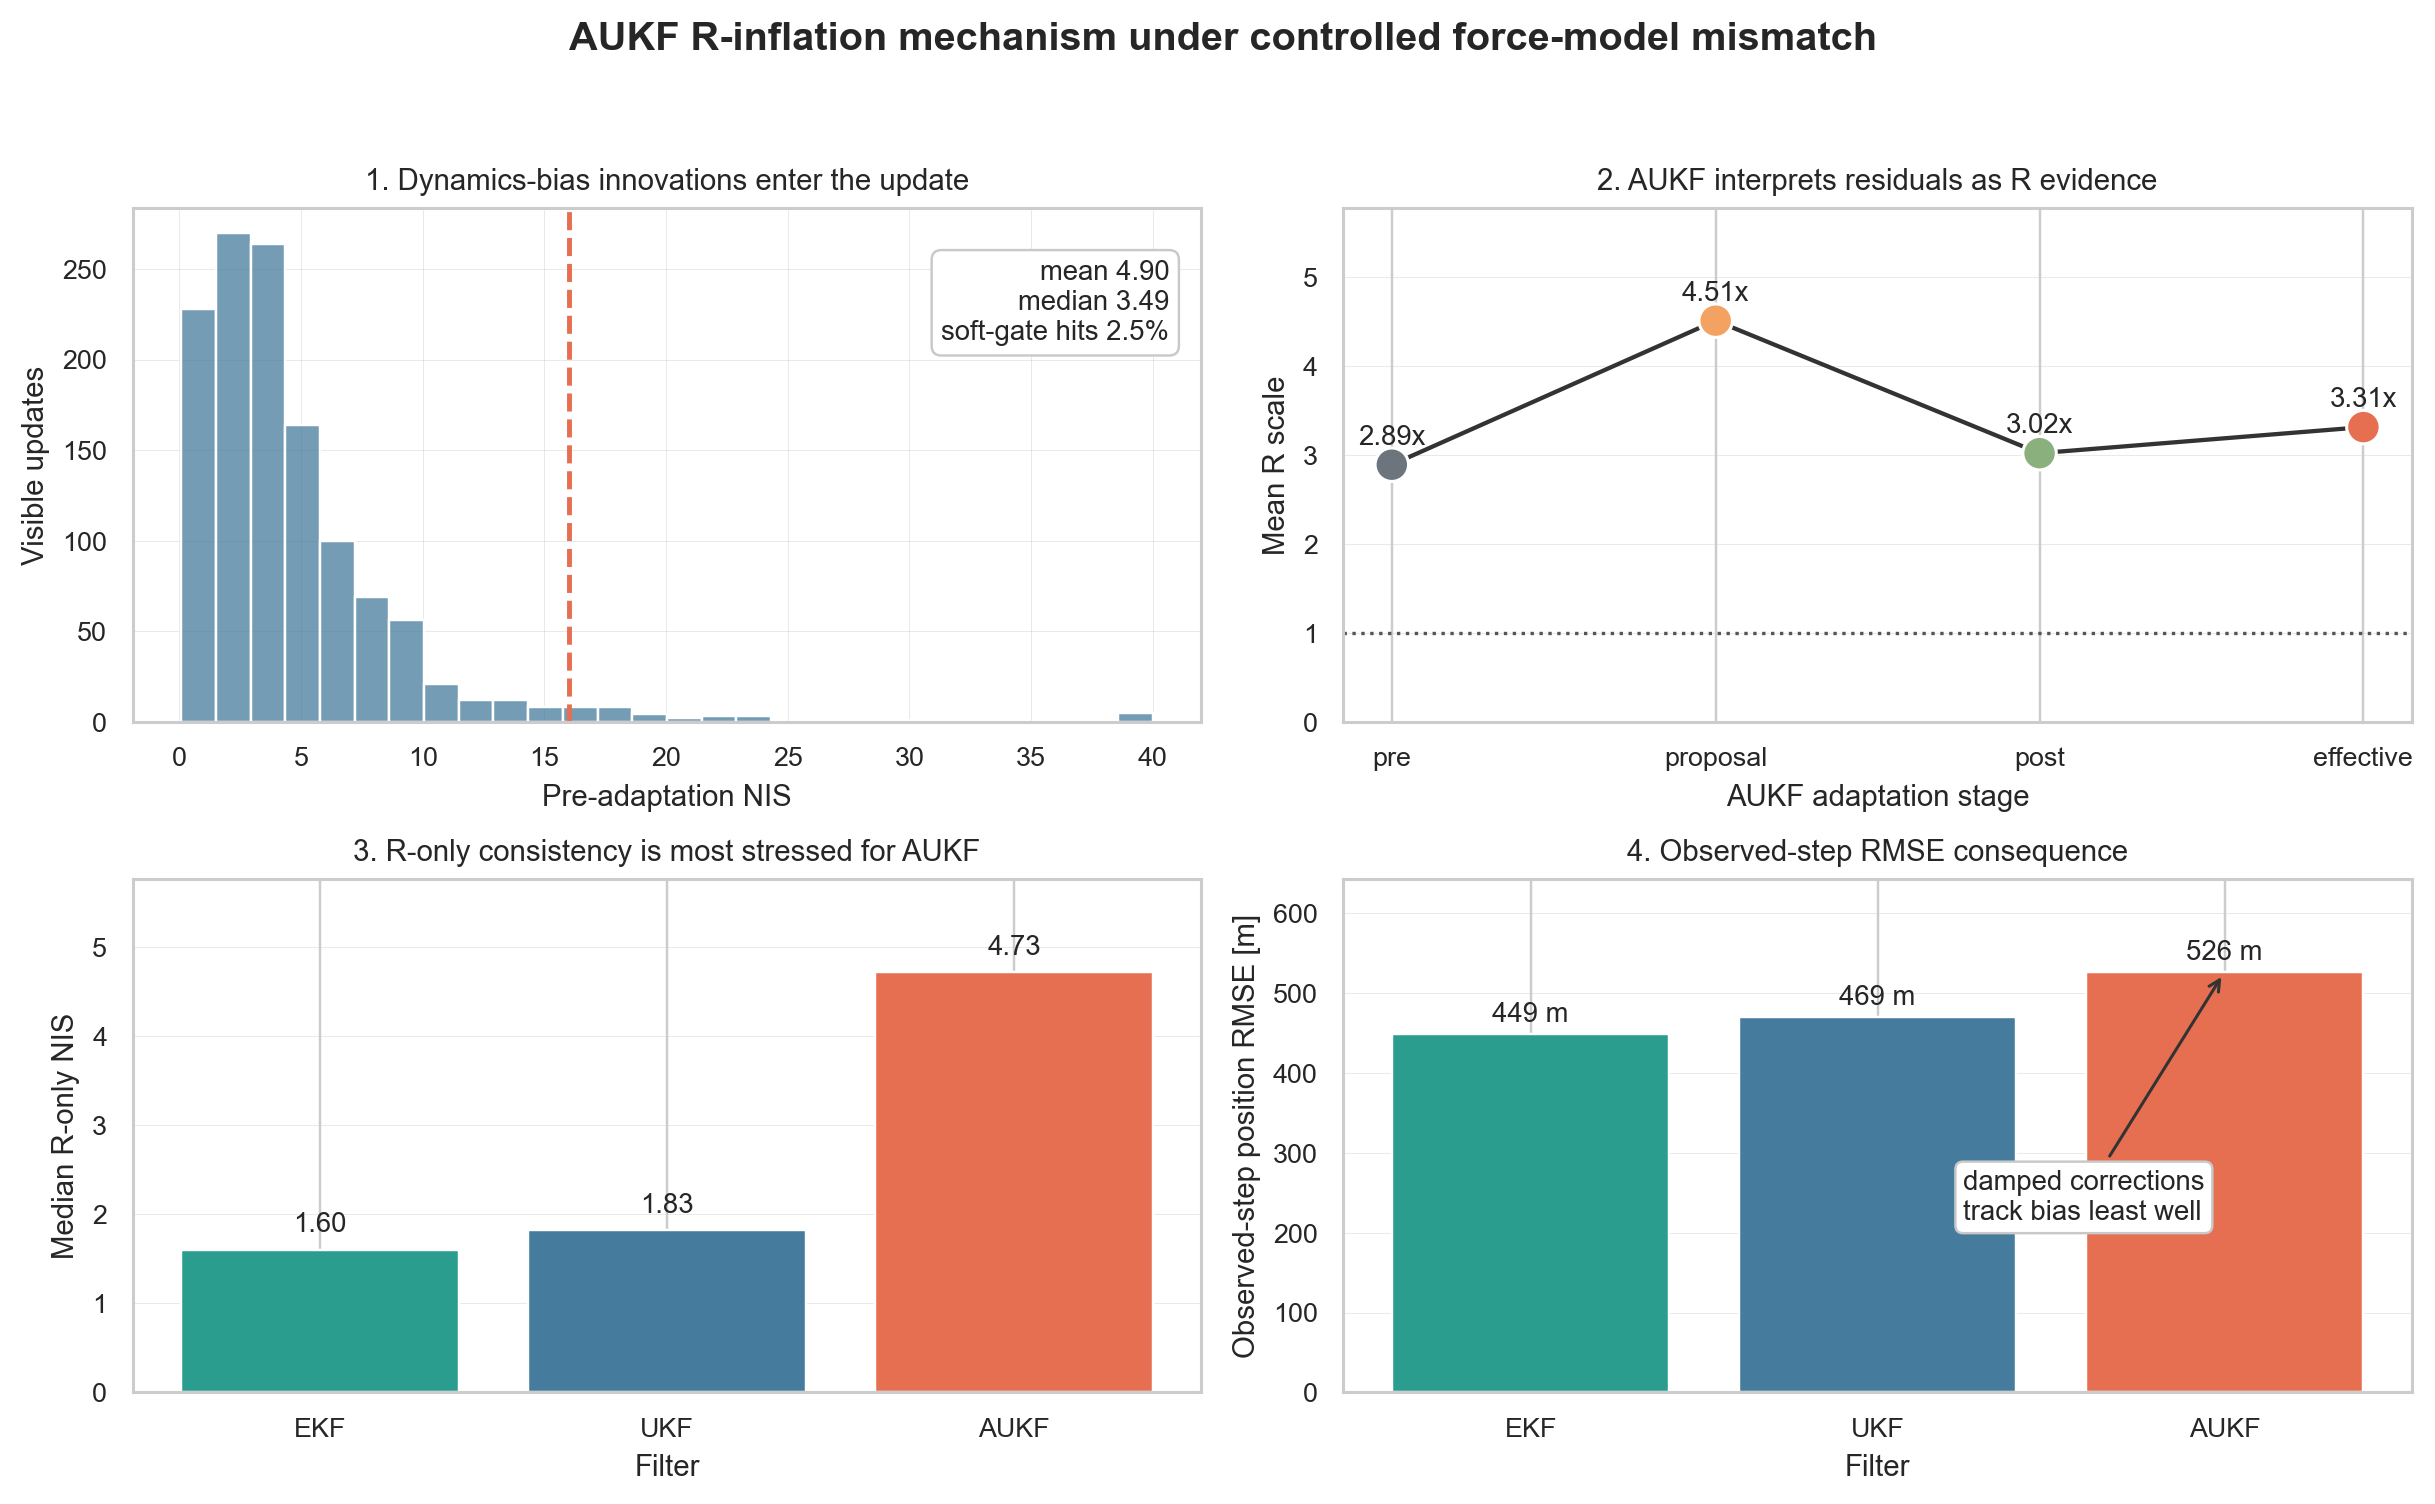
\includegraphics[width=\linewidth]{figures/aukf_r_inflation_mechanism.png}
  \caption{Main-text mechanism view of the controlled force-model-mismatch AUKF diagnostic. Dynamics-bias innovations raise the adaptation signal, and the AUKF inflates effective \(R\) (mean scale 3.32, from 2.89) while EKF and UKF remain near nominal scale (mean 1.00, 0.99 respectively). Median \(R\)-only NIS grows from 1.60 (EKF) and 1.83 (UKF) to 4.73 (AUKF), and AUKF shows worse observed-step position RMSE than the fixed-noise references on this force-mismatch slice. The figure is derived from the same deterministic compact-model force-mismatch diagnostic summarized in Table~\ref{tab:main_aukf_mechanism} and S-Table~\ref{tab:force_mismatch_mechanism}, not from a new run.}
  \label{fig:aukf_r_inflation_mechanism}
\end{figure}

\begin{table}[t]
  \centering\small
  \caption{Compact-model AUKF mechanism diagnostic on the controlled force-model mismatch. The deterministic decomposition reproduces the reference AUKF estimate to 0.00 m and shows the known covariance-matching failure mode in OD form: dynamics-bias innovations are treated as measurement-noise evidence, inflating effective \(R\) and damping the updates needed to track the biased truth. Values are aggregated over the full controlled force-mismatch mechanism population (48 processed trajectories); visible-update counts and update-norm statistics are computed over the visible AUKF update records in that population.}
  \label{tab:main_aukf_mechanism}
  \resizebox{\linewidth}{!}{%
  \begin{tabular}{lc}
    \toprule
    Diagnostic quantity & Value \\
    \midrule
    Visible measurement updates & 1238 \\
    Pre-adaptation NIS (mean / median / p90) & 4.90 / 3.49 / 9.16 \\
    Effective \(R\) scale (pre / proposal / post / effective) & 2.891 / 4.513 / 3.021 / 3.315 \\
    Mean state-update norm [m] & 466.31 \\
    \(R\)-only median NIS (EKF / UKF / AUKF) & 1.60 / 1.83 / 4.73 \\
    AUKF \(R\)-only p90 NIS & 20.38 \\
    Observed-step RMSE (EKF / UKF / AUKF) [m] & 448.79 / 469.41 / 526.39 \\
    AUKF estimate max position difference vs reference [m] & 0.00 \\
    \bottomrule
  \end{tabular}
  }
\end{table}

As an additional targeted mechanism-control, S-Table~\ref{tab:constrained_aukf_mechanism_control} runs AUKF with effective \(R\) scale capped at \(2\times\) nominal (AUKF-Rcap) across all 48 force-mismatch trajectories. AUKF-Rcap inherits all standard AUKF parameters unchanged and differs only in the maximum effective \(R\)-scale ceiling, which is reduced from 30$\times$ to 2$\times$. All 48 trajectories are processed; the paired denominator is 38 because 10 trajectories have zero visible measurements after the scoring window starts at step~11, making observed-step trajectory RMSE undefined for all comparators under the shared visibility/scoring mask---these are not AUKF-Rcap- or standard-AUKF-specific nonfinite failures. All paired CIs and win rates are computed over the 38 shared finite observed-step trajectories. Capping the inflation reduces the mean effective \(R\) scale from 3.32 to 1.09 and improves the pooled observed-step RMSE by 41.7~m relative to standard AUKF (paired gap $-23.6$~m, 95\% CI $[-42.3, -6.2]$~m; 63.2\% win rate over 38 paired finite trajectories, above the 50\% equal-direction reference; this is an additional targeted mechanism-control outside the original frozen learned-estimator claim audit and not a predeclared positive criterion). AUKF-Rcap remains strictly worse than EKF ($+34.5$~m, CI $[+9.8, +63.9]$~m), supporting the interpretation that \(R\)-inflation damping is a key but not sole driver of the AUKF degradation under compact-model dynamics bias.

As a post-review exploratory guard against reading the mechanism as a single-slice anecdote, two cross-scenario diagnostics separate an older cached-prediction residual readback from a stricter true pre-update innovation readout. The cache-busted 17-scenario readback recomputes observed-step EKF/UKF/AUKF RMSE from fresh baseline caches and computes a cached-prediction \(R\)-only NIS ratio \(\rho_{\mathrm{NIS}}=\mathrm{median\,NIS}_{\mathrm{AUKF}}/\mathrm{median\,NIS}_{\mathrm{UKF}}\). It is not predeclared, not a confirmatory classifier, and not operational POD; it is retained only as hypothesis-generating mechanism support. In that bounded readback, AUKF is worse than fixed-noise UKF in 6/17 scenarios and worse than the better non-adaptive EKF/UKF reference in 12/17 scenarios. The high-ratio rule \(\rho_{\mathrm{NIS}}\geq1.25\) has 4/4 precision and 4/6 recall for AUKF-worse-than-UKF, and 4/4 precision but only 4/12 recall for AUKF-worse-than-best-nonadaptive; Wilson intervals are [0.51, 1.00] for precision, [0.30, 0.90] for UKF recall, and [0.14, 0.61] for best-nonadaptive recall. Recomputing \(R\)-only NIS on all trajectories preserves the retained-threshold classification, so the cached-prediction result supports the narrow interpretation that elevated residual stress can warn of adaptive-\(R\) underperformance, while explicitly failing to validate a transferable decision rule.

The stricter follow-up uses a fixed 10-cell synthetic scenario frame, eight independent fresh realizations per cell, and 12 trajectories per realization (80 finite rows, 960 trajectories, and 22,574 observed steps; \nolinkurl{results/aukf_nis_sampled_campaign/aukf_pre_update_nis_sampled_campaign_k8_n12_20260616.md}). The diagnostic \(\rho_{\mathrm{pre}}\) is computed from true pre-update \(R\)-only innovation records emitted inside the UKF and AUKF recursions immediately before each visible station update, so it is not reconstructed from post-update stored filter histories. At \(\rho_{\mathrm{pre}}\geq1.25\), the warning fires on only 8/80 rows. For AUKF-worse-than-UKF, it records 6 true positives, 2 false positives, and 31 false negatives: precision 6/8 = 0.75 (Wilson 95\% CI [0.41, 0.93]) and recall 6/37 = 0.16 (CI [0.08, 0.31]). For AUKF-worse-than-best-nonadaptive, it records 8/8 precision (CI [0.68, 1.00]) and 8/52 recall (CI [0.08, 0.28]). Lowering the threshold to 1.10 raises recall but admits more positives: best-nonadaptive precision is 15/16 (CI [0.72, 0.99]) with 15/52 recall (CI [0.18, 0.42]), and UKF-specific precision is 12/16 (CI [0.51, 0.90]) with 12/37 recall (CI [0.20, 0.49]). Thus the pre-update ratio is a high-specificity, low-recall stress warning in this internal sampled frame, not a calibrated classifier and not evidence of operational transfer.

A higher-fidelity pre-update repeat then tests the same true-recursion diagnostic outside the compact scenario frame without adding learned models or retuning filters (\nolinkurl{results/hifi_pre_update_nis_campaign/hifi_pre_update_nis_campaign_base_extended_k8_n12_20260616.md}). It uses two high-fidelity truth cells, J2..J4+third-body and J2..J6+third-body+diurnal-density truth, with eight independent realizations per cell and 12 trajectories per realization (16 finite rows, 192 trajectories, 4,482 observed steps, no divergent rows). The diagnostic collapses near unity (median \(\rho_{\mathrm{pre}}=0.990\), range 0.956--1.019), so the thresholds 1.10, 1.25, and 1.50 fire on zero rows. This silence misses every underperformance case in the repeat: AUKF is worse than UKF on 7/16 rows and worse than the best nonadaptive EKF/UKF reference on 10/16 rows. The repeat therefore falsifies a transferable-threshold reading of the compact warning; it supports only the narrower statement that high \(\rho_{\mathrm{pre}}\) was a sparse, high-specificity warning in the sampled compact frame.

Reading the compact force-mismatch diagnostic, the cache-busted readback, the higher-fidelity pre-update repeat, the long-arc higher-fidelity slice, and the drag-scale cascade as a regime matrix clarifies the claim. The compact slice is the only row where the AUKF warning is load-bearing: \(\rho_{\mathrm{NIS}}\approx2.59\), AUKF has the highest observed-step RMSE among EKF/UKF/AUKF, and effective-\(R\) inflation is directly visible. In the two-cell higher-fidelity pre-update repeat, \(\rho_{\mathrm{pre}}\) stays near one and misses AUKF-worse labels; in the 3-hour higher-fidelity row, \(\rho_{\mathrm{NIS}}\approx1.03\), AUKF is the best non-DSA estimator, and DSA-EKF still fails. Thus neither the compact EKF-over-AUKF ordering nor the compact warning threshold transfers. The drag-scale rows then localize a different structural failure: EKF augmentation fails by linearisation, UKF augmentation removes the catastrophe but leaves \(\hat\beta\) near one, and the dense 12-hour row leaves \(\hat\beta\) near one even with kilometre-scale drag separation. The contribution is therefore a bounded mechanism map for escalation decisions, not a transferable AUKF rejection rule.

\subsection{Higher-fidelity force-mismatch (second-fidelity scoping)}\label{sec:hifi-force-mismatch}
Higher-fidelity force-mismatch slices preserve the \(R\)-only NIS stress signature but do not support transferring the compact EKF-over-AUKF ordering.
S-Table~\ref{tab:hifi_force_mismatch} repeats the controlled force-mismatch protocol with the truth-side dynamics extended above the compact-J2 ceiling: the truth propagator adds the J3 and J4 zonal geopotential terms (analytic gradient of the standard zonal expansion) and luni-solar third-body acceleration (analytic low-precision ephemerides at absolute UTC epoch), while every estimator still keeps the nominal compact two-body+$J_2$+drag model. On this richer dynamics mismatch the cross-filter $R$-only NIS diagnostic of S-Table~\ref{tab:force_mismatch_mechanism} continues to fire (AUKF median $R$-only NIS $1.53$ vs.\ EKF $1.37$ and UKF $1.47$, AUKF p90 $5.70$), so the compact-model mechanism reproduces qualitatively. The magnitude of the AUKF damping is, however, no longer load-bearing in the EKF$/$AUKF comparison: the tuned AUKF is the best classical filter ($393.3$~m mean observed-step RMSE), the causal EKF is second ($420.9$~m), and the EKF$-$AUKF paired-bootstrap CI spans zero ($[-152.5, +243.8]$~m). The predeclared PUKF again fails its positive criterion (significantly worse than AUKF by $+126.4$~m, CI $[+14.9, +296.3]$~m; Section~\ref{sec:pukf}, S-Table~\ref{tab:pukf_force_mismatch}). The AUKF caveat from S-Table~\ref{tab:force_mismatch_mechanism} is therefore a \emph{compact-model} observation: above the compact-J2 ceiling the mechanism continues to fire but the EKF$/$AUKF ordering is not flipped, so we downscope the compact-model diagnostic. A yet richer fidelity slice (S-Table~\ref{tab:hifi_force_mismatch_extended}, J5$+$J6 zonal terms plus a one-sided diurnal-bulge density modulation, $\alpha=0.30$) confirms the same downscoping: the cross-filter $R$-only NIS again flags AUKF as the most stressed (median $1.67$ vs.\ EKF $1.42$, UKF $1.60$) but the EKF$/$AUKF ordering does not flip (EKF$-$AUKF mean $-21.3$~m, CI $[-160.4, +87.1]$~m spans zero), and the best classical filter is the fixed-noise UKF rather than EKF.

\subsection{Process Noise Adaptive UKF (predeclared)}\label{sec:pukf}

PUKF fails its predeclared positive criterion on both the controlled compact and higher-fidelity force-mismatch slices.
S-Table~\ref{tab:pukf_force_mismatch} reports the \emph{predeclared symmetric Q-adaptive UKF (PUKF)} on the same 38-trajectory controlled force-mismatch population. The rule, thresholds, and decision predicate (PUKF is a positive contribution iff its mean observed-step RMSE is strictly lowest and the paired-bootstrap CI versus every comparator is strictly below zero) were predeclared in a timestamped rule record before the evaluation; no rule retuning is allowed. Outcome: PUKF inflates the predicted process covariance heavily (mean $\bar Q$-scale $5.9$) but does \emph{not} satisfy the predeclared positive criterion --- its mean observed-step RMSE is worse than the causal EKF ($+42.6$~m, CI $[+15.4,+74.0]$~m), and the CI versus tuned UKF spans zero ($+16.5$~m, CI $[-7.0,+38.8]$~m). On the higher-fidelity slice (S-Table~\ref{tab:hifi_force_mismatch}) the predeclared positive criterion likewise fails (PUKF significantly worse than AUKF, CI $[+14.9,+296.3]$~m). A post-hoc 16-point validation-grid stress for PUKF on that higher-fidelity slice (S-Table~\ref{tab:pukf_tuning_sensitivity}) also does not rescue the comparator: the PUKF selected on validation data remains worse than AUKF on the retained held-out population (selected PUKF $527.5$~m vs.\ AUKF $393.3$~m; paired gap $+134.2$~m, CI $[-9.5,+382.2]$~m over $n=38$ finite paired trajectories). The drag-scale cascade supplement also records a separate 12-hour observability-grid case in which PUKF overflows on the unaugmented UKF-family stress slice; that is a scope warning for long-arc sigma-point conditioning, not part of the predeclared 40-minute PUKF decision. Because this CI spans zero and is wide, the sensitivity supports only the qualitative conclusion that this bounded validation grid does not rescue PUKF; it does not establish a tuning-sensitive ordering. This sensitivity is reported for tuning comparability only and does not replace the predeclared PUKF evidence. PUKF is therefore a \emph{predeclared bounded negative} at both fidelities, with an added post-hoc comparability stress, and the remaining diagnostic focus is structural (Sections~\ref{sec:dmc-ekf}, \ref{sec:dsa-ekf}) rather than statistical noise adaptation alone.

\subsection{Predeclared Cartesian structural-channel response (DMC-EKF)}\label{sec:dmc-ekf}
The compact DMC-EKF structural-channel check does not beat UKF on the higher-fidelity force-mismatch slice.
Stacey and D'Amico's 2021 adaptive, dynamically constrained process-noise OD work motivates structural process-noise responses to dynamics/force-model bias; the DMC/DSA implementations here are compact, simplified structural-channel checks motivated by that lineage, not faithful reproductions of the full adaptive dynamically constrained formulation and not a rejection of that broader prescription~\cite{stacey2021adaptive}.

Section~\ref{sec:pukf} reports a predeclared symmetric $Q$-adaptive UKF (PUKF) as the statistical counterpart of the innovation-adaptive AUKF; both PUKF and AUKF adapt the noise distribution on the $R$ or $Q$ side without changing the deterministic flow. Classical statistical OD prescribes a complementary \emph{structural} response when the dominant residual is a dynamics/force-model bias: augment the state with a low-frequency empirical-acceleration channel and estimate it jointly with position and velocity, the dynamic model compensation (DMC) recipe \cite{tapley2004statistical,wright1981drag,stacey2021adaptive}. S-Table~\ref{tab:dmc_ekf_force_mismatch} reports the predeclared DMC-EKF on the higher-fidelity force-mismatch slice (truth-side J2..J6 zonal geopotential plus luni-solar third-body plus one-sided diurnal-bulge atmospheric-density modulation; estimators on the compact two-body+$J_2$+drag deterministic flow). The augmented state appends a per-axis first-order Gauss--Markov empirical-acceleration channel $w$ with predeclared steady-state standard deviation $\sigma_w=1.0\times10^{-6}~\text{m/s}^2$ and decorrelation time $\tau=300$~s; the deterministic flow is shared with the EKF baseline. The predeclared positive criterion (DMC-EKF strictly lowest in mean observed-step RMSE, strictly negative paired-bootstrap CI versus the best non-DMC comparator, and the 3\% practical significance floor exceeded) was committed in a timestamped rule record, and no rule retuning is allowed. Outcome: the predeclared criterion is \emph{not} satisfied --- UKF gives the lowest mean ($276.13$~m), DMC-EKF tracks EKF to numerical precision (paired mean difference $7.8\times10^{-6}$~m), and the DMC-EKF$-$UKF paired-bootstrap CI spans zero ($+2.9$~m vs.\ UKF, $[-3.8, +8.1]$~m). The cause is structural: under sparse-visibility geometry the empirical-acceleration channel is essentially observable only through position/velocity cross-covariance accumulated between visible updates, and the median maximum estimated $|w|$ remains near $1\times10^{-10}~\text{m/s}^2$, far below the unmodeled-physics magnitude. The near-zero DMC-EKF--EKF deviation is consistent with the sparse-visibility observability bound rather than with a process-covariance-augmentation implementation defect: a separate favorable-geometry sanity diagnostic in S-Table~\ref{tab:structural_channel_recoverability} shows that the same DMC-EKF empirical-acceleration channel recovers a known matched acceleration vector to 2.15\% relative error and lowers RMSE relative to EKF when all stations are visible and measurement noise is intentionally low. We report this as a \emph{predeclared Cartesian-structural-channel bounded negative}: the standard structural response to dynamics bias does not transfer to this sparse-visibility regime under the predeclared rule, so the audit returns a bounded negative on both the noise-adaptive family (AUKF, PUKF) and the Cartesian structural-channel family (DMC-EKF) on the higher-fidelity slice. This strengthens the audit's scope: the compact-model AUKF mechanism diagnostic is not rescued by the canonical Cartesian structural channel above the compact-$J_2$ ceiling under sparse visibility.

\subsection{Predeclared parametric structural-channel response (DSA-EKF)}\label{sec:dsa-ekf}
DSA-EKF gives a statistically detectable but below-floor improvement on the 40-minute higher-fidelity slice, so it remains a predeclared negative.
One diagnostic concern for the Cartesian channel of Section~\ref{sec:dmc-ekf} is that a generic per-axis empirical acceleration may be the less specific structural channel for the actual mismatch (drag/density/ballistic-coefficient bias); the standard LEO structural recipe estimates the multiplicative \emph{drag-scale} parameter directly~\cite{tapley2004statistical,wright1981drag,lowe2026drag}; learned per-satellite drag-coefficient estimation has also been pursued for OD and prediction~\cite{chen2025bilstmdrag}, whereas the diagnostic here shows a parametric drag-scale channel is inert under sparse visibility. S-Table~\ref{tab:drag_scale_aekf_force_mismatch} reports the predeclared seven-state DSA-EKF on the same higher-fidelity slice as DMC-EKF: the augmented state is $[r, v, \beta]$ with $\beta$ a first-order Gauss--Markov drag-scale parameter about its nominal value of one, and the deterministic flow scales the drag acceleration by $\beta(t)$ on top of the otherwise compact two-body+$J_2$+drag model. The Gauss--Markov hyperparameters were selected on a disjoint validation seed over a four-point predeclared grid before the held-out test; the selection record and timestamped rule are retained for inspection. The predeclared positive criterion (DSA-EKF strictly lowest in mean, strictly negative paired CI versus the best non-DSA comparator, gap above the 3\% practical significance floor defined in the statistical protocol) is \emph{not} satisfied: DSA-EKF gives the lowest mean ($347.67$~m versus EKF $354.69$~m), and the DSA-EKF$-$EKF paired-bootstrap CI is strictly below zero ($-7.0$~m, $[-9.7, -4.8]$~m), but the absolute gap lies \emph{below the predeclared $10.6$~m floor}. The associated Wilcoxon signed-rank descriptive $p$-value on the same pairing is highly significant ($p\approx 1.8\times 10^{-9}$); we report this as an explicit illustration of the manuscript's predeclared posture that \emph{statistical detectability is not the same as practical significance} --- a strictly negative paired CI versus the EKF coexists here with a reported, statistically robust within-floor improvement of about $7$~m, and the predeclared rule therefore returns a bounded negative regardless of the underlying $p$-value. A below-floor strictly-negative CI of this kind does not imply that the structural channel provides \emph{zero} benefit; below-floor is not the same as inert, but it is also not a positive contribution under the predeclared rule because the measured benefit is smaller than the practical significance threshold. The estimated drag-scale parameter moves by only $|\hat{\beta}-1|\sim 10^{-7}$ from its prior over the 40-minute filter window, confirming that the parametric channel is essentially unobservable from sparse line-of-sight measurements at this window length: insufficient drag-induced orbit decay accumulates in 40~min to constrain $\beta$. We report this as a \emph{predeclared parametric-structural-channel bounded negative} alongside the Cartesian DMC bounded negative, so the audit closes both standard structural responses to dynamics bias under sparse visibility, not only one.

\subsection{Structural-channel sanity and drag-scale cascade}\label{sec:drag-scale-cascade}
Favorable-geometry checks show the structural channels can recover matched signals, while the three-slice cascade still returns bounded negatives and localizes the drag-scale failure modes.
Before interpreting the sparse-visibility structural-channel negatives, Table~\ref{tab:main_structural_recoverability} records the favorable-geometry sanity check that the implemented DSA-EKF drag-scale channel and DMC-EKF empirical-acceleration channel can recover matched known signals under intentionally easy measurements. This is not a primary endpoint and not an operational OD result; it is a positive implementation check showing that the later negatives are not caused by a structural-channel implementation that cannot move under any geometry.

\begin{table}[t]
  \centering\scriptsize
  \caption{Main structural-channel implementation sanity check. The favorable-geometry diagnostic is not a primary endpoint and not an operational OD case; it brackets the sparse-visibility negatives by showing that the implemented structural channels can recover matched known signals when the measurement geometry is intentionally easy.}
  \label{tab:main_structural_recoverability}
  \begingroup\setlength{\tabcolsep}{3pt}
  \begin{tabular}{@{}p{0.17\linewidth}p{0.19\linewidth}p{0.23\linewidth}p{0.13\linewidth}p{0.20\linewidth}@{}}
    \toprule
    Channel & Known signal & Last-window estimate & EKF$\to$channel RMSE [m] & Readout \\
    \midrule
    DSA-EKF drag scale & $\beta=4.00$ & $\hat\beta=3.981$; 0.46\% error & 0.72$\to$0.71 & Matched beta channel recovers under all-visible, low-noise geometry. \\
    DMC-EKF empirical acceleration & $[2.00, -1.00, 1.50]\times10^{-5}$ & $[2.02, -1.05, 1.50]\times10^{-5}$; 2.15\% error & 4.20$\to$3.45 & Matched acceleration channel recovers under the same sanity regime. \\
    \bottomrule
  \end{tabular}
  \endgroup
\end{table}

Table~\ref{tab:main_drag_scale_cascade} then gives the three-slice drag-scale mechanism cascade. The first slice fixes the structural form to the true multiplicative drag-scale bias and identifies EKF analytic linearisation as the binding failure mode for the EKF-based candidate. The second slice substitutes deterministic sigma-point propagation of the augmented flow, removes that failure mode, and leaves a separate sparse-visibility observability-side bound: DSA-UKF is near UKF/AUKF in RMSE but $\hat{\beta}$ remains effectively at one. The third slice enriches the geometry and extends the arc; even with 9.6 km median arc-mean drag-induced separation, median trajectory-mean \(\hat{\beta}=1.0000\) and median maximum \(|\hat{\beta}-1|=0.0010\), isolating candidate-side \(\beta\) prior inertia while also stressing the unaugmented UKF-family baselines. We therefore read the third row as a candidate-side beta-inertia diagnostic plus a long-arc sigma-point-stress record, not as a well-conditioned UKF-family ranking. This three-way mechanism separation---linearisation, observability, and candidate-side prior inertia---is the paper's central non-self-referential diagnostic: it localises the structural-channel failure to a specific binding constraint rather than re-measuring a known mode. The inertia is consistent with an identifiability argument: the line-of-sight innovation is absorbed by the well-observed position/velocity correction while \(\beta\) enters only through twice-integrated drag, so the minimum-variance update attributes a position offset to \(r,v\) rather than to \(\beta\), and the favorable-geometry sanity check (Table~\ref{tab:main_structural_recoverability}) recovers \(\beta\) precisely because that aliasing is suppressed. The full grid and stability caveats are in supplementary Section~\ref{app:observability-positive-control-ukf}.

\begin{table}[t]
  \centering\scriptsize
  \caption{Main mechanism cascade for the drag-scale structural channel. Positive candidate-minus-reference gaps mean the candidate is worse than the best eligible reference. All three rows use held-out test populations after the relevant selection rule is frozen; none satisfies its predeclared positive criterion.}
  \label{tab:main_drag_scale_cascade}
  \begingroup\setlength{\tabcolsep}{3pt}
  \begin{tabular}{@{}p{0.15\linewidth}p{0.18\linewidth}p{0.18\linewidth}p{0.19\linewidth}p{0.20\linewidth}@{}}
    \toprule
    Slice & Observed-step RMSE comparison [m] & Candidate$-$reference [m] (95\% CI) & Drag-scale response & Mechanism readout \\
    \midrule
    Matched channel, EKF predict & DSA-EKF 1648.5 vs UKF 359.7 & $+1288.9$ [$+378.1$, $+2561.4$] & max $|\hat{\beta}-1|=0.0012$; final $\hat{\beta}=1.0000$ & Structural form is matched, but the EKF predict step is the binding failure mode. \\
    Sigma-point substitution & DSA-UKF 316.4 vs AUKF 313.1 & $+3.3$ [$-7.5$, $+16.2$] & max $|\hat{\beta}-1|=0.0009$; final $\hat{\beta}=1.0000$ & Sigma-point propagation removes the EKF divergence but not the AUKF guardrail. \\
    Geometry-enriched DSA-UKF & DSA-UKF 4879.9 vs EKF 742.7 & $+4137.2$ [$-827.0$, $+11235.7$] & max $|\hat{\beta}-1|=0.0010$; final $\hat{\beta}=1.0000$ & Drag signal is visible (9595.9 m mean, 29294.1 m final), but estimated $\hat{\beta}$ remains inert; UKF-family baselines are long-arc stressed, so this row is not a stable UKF ranking. \\
    \bottomrule
  \end{tabular}
  \endgroup
\end{table}

\subsection{Long-arc higher-fidelity force-and-density-mismatch replication}\label{sec:long-arc-hifi}
Extending the arc to three hours does not rescue DSA-EKF; it is still worse than AUKF and the drag-scale state moves only marginally.

A practical concern on the 40-minute higher-fidelity slice is that the drag-scale structural channel may simply remain unobservable over such a short window. We therefore run a \emph{long-arc higher-fidelity force-and-density-mismatch replication} (Table~\ref{tab:main_long_arc_result}; S-Table~\ref{tab:long_arc_hifi_force_mismatch}) with a 3-hour arc, richer truth-side force and density mismatch, and the same compact estimator-side dynamics. DSA-EKF hyperparameters are selected on a disjoint long-arc validation seed before held-out testing.

The decision floor is an approximate astrodynamics-grounded Cram\'er--Rao position floor under the configured geometry and stated independence assumptions. The supplement gives the derivation and sensitivity audit using Tapley--Schutz--Born statistical OD theory~\cite{tapley2004statistical}. The resulting 106.0~m floor is unchanged when range-rate noise is added as a worst-case perturbation check, so the floor is not being set by an omitted range-rate term.

The substantive result is negative for transfer: even on the longer, richer slice DSA-EKF remains worse than AUKF, and the drag-scale state still shows only marginal movement. We therefore read this slice as a higher-fidelity long-arc failure-to-transfer result, not as evidence that the compact-$J_2$ EKF-over-AUKF ordering generalizes. The detailed interval and stability audit remains in the supplement.

\begin{table}[t]
  \centering\small
  \caption{Long-arc higher-fidelity force-and-density-mismatch result. DSA-EKF fails its predeclared positive criterion because AUKF is the best non-DSA estimator and the DSA-EKF$-$AUKF interval is positive. The auxiliary EKF/AUKF stress observation is retained only as supplementary stress context.}
  \label{tab:main_long_arc_result}
  \resizebox{\linewidth}{!}{%
  \begin{tabular}{lcccccc}
    \toprule
    Quantity & EKF & UKF & AUKF & PUKF & DMC-EKF & DSA-EKF \\
    \midrule
    Mean observed-step RMSE [m] & 577.05 & 345.05 & \textbf{312.66} & 405.98 & 577.05 & 597.09 \\
    \bottomrule
  \end{tabular}
  }
  \\[2pt]{\footnotesize Held-out \(n=64\). DSA-EKF$-$AUKF mean \(+284.4\) m, CI \([+8.7,+697.9]\) m. The predeclared CRLB floor is 106.0 m and treats visible steps as independent; this can tighten the floor under within-pass correlation. The supplement reports a 36.8--335.1 m sensitivity range; pass-correlated S-Table row F is the opposite-direction bound at 335.1 m. Decision unchanged because DSA-EKF fails direction before floor magnitude under every variant.}
\end{table}

\subsection{KalmanNet linear-canonical sanity reproduction}\label{sec:kalmannet-faithful}

The official KalmanNet linear-canonical sanity check (S-Table~\ref{tab:kalmannet_official_reproduction}) reproduces the published release \cite{revach2022kalmannet} at reduced scale and confirms the trained KalmanNet sits within $0.2$~dB of the optimal Kalman filter on its own native benchmark. The load-bearing learned-claim comparator for this paper's bounded negative remains the in-house KalmanNet-style learned-gain comparator (S-Table~\ref{tab:kalmannet_gain_inhouse_comparator}). The manuscript also reports a separately predeclared KalmanNet SPOT-OD transposition under four documented adaptations---orbital-scale normalization, full-arc curriculum rematching, sparse-observation masking, and lower-rate budget recalibration---as a feasibility note for readers who would otherwise ask whether the external architecture was tried at all (supplementary Section~\ref{app:kalmannet-spot-od-transposition}, S-Tables~\ref{tab:kalmannet_spot_od_transposition}--\ref{tab:kalmannet_spot_od_budget_adequacy}). Under that transposition, the upstream gain network remains far above the best classical reference on the held-out SPOT-OD test population even after a six-fold budget extension from 300 to 1800 optimizer steps: mean observed-step RMSE descends from 152.7~km to 136.0~km, while the best classical reference (AUKF) remains 340.9~m and the validation-best 1200-step snapshot still sits at 139.1~km. Because that gap is still consistent with an undertrained or mismatched transposition, we report it only as bounded feasibility evidence for this documented adaptation and budget schedule, not as load-bearing evidence for the paper's learned-negative claim and not as an architecture-level conclusion.\label{sec:kalmannet-spot-od}

\subsection{DBAR (predeclared heuristic, withdrawn)}\label{sec:dbar-withdrawal}
DBAR is withdrawn because the powered simulator characterization does not exceed its no-information baseline and the compact public SP3 replay does not transfer.

The mechanism diagnostic motivated a predeclared decision rule for the Dynamics-Bias Adaptation-Risk (DBAR) indicator. On the powered 450-realization simulator characterization, DBAR is not statistically distinguishable from its $81.3\%$ no-information majority baseline because the Wilson 95\% interval still contains that baseline.

The public precise-reference probe is also negative. The original ten-arc LAGEOS diagnostic reaches only 6/10 correct, below the 0.80 always-no-fire majority baseline. The stronger result is the formal 400-arc compact recursive-filter replay: 400 arcs were attempted, 373 completed, and 27 are carried as explicit status records rather than hidden or imputed (17 insufficient observations; 10 public product unavailable or non-parseable).

On the 373 completed arcs, DBAR is correct on 256/373 arcs (0.686), below the 0.737 no-fire majority baseline, with sensitivity 0.480 and specificity 0.760. Pooled held-out RMSE is EKF 566.60~m, fixed-noise UKF 573.24~m, AUKF 601.38~m, and SP3-IC propagation 779.45~m. Under the first-minus-second convention, EKF-minus-AUKF has mean $-34.78$~m, median $-0.76$~m, and 95\% CI $[-71.84,-2.76]$~m, while fixed-noise-UKF-minus-AUKF has mean $-28.14$~m, median $-0.77$~m, and CI $[-61.80,-2.75]$~m; both intervals therefore indicate larger held-out RMSE for AUKF on average.

The practical interpretation is narrow. DBAR remains a useful predeclared stress test because it produced a clear negative and forced explicit withdrawal, but it is not promoted as a transferable decision statistic. Table~\ref{tab:main_dbar_withdrawal} and Section~\ref{sec:claim-audit} define the final scope.

\begin{table}[t]
  \centering\small
  \caption{Powered DBAR characterization and withdrawal. DBAR does not beat the no-information majority classifier after 450 independently seeded realizations, so the heuristic is withdrawn as a claimed positive and retained only as a characterized negative.}
  \label{tab:main_dbar_withdrawal}
  \resizebox{\linewidth}{!}{%
  \begin{tabular}{lcccc}
    \toprule
    Regime family & \(N\) & DBAR fires & \(R\)-adaptation bad & Accuracy \\
    \midrule
    Nominal control & 150 & 0 & 14 & 90.7\% \\
    Measurement-noise stress & 150 & 10 & 6 & 89.3\% \\
    Dynamics/force-model bias & 150 & 104 & 64 & 65.3\% \\
    \midrule
    \textbf{All} & 450 & 114 & 84 & \textbf{81.8\%} \\
    \bottomrule
  \end{tabular}
  }
  \\[2pt]{\footnotesize The always-no-fire majority baseline is 81.3\%; DBAR's \(+0.4\)-point increment has Wilson 95\% interval \([78.0,85.1]\%\) containing the baseline. The predeclared rule is therefore not a validated classifier.}
\end{table}

\subsection{Multi-revolution SGP4-reference benchmark}
The public-catalog multi-revolution stress keeps recursive filters at kilometre scale and the learned residual worse than the best classical filter.
The \emph{multi-revolution SGP4-reference state-error benchmark} with \emph{real ground-station geometry} (five real public LEO objects, SGP4-propagated reference from archived CelesTrak TLEs, 12-hour 7.07--7.81-revolution arcs, sparse line-of-sight measurements from the real eight-station geometry, every estimator on the compact two-body+$J_2$+drag OD model, so \emph{the SGP4 reference is a genuine multi-revolution dynamics-model mismatch}; S-Table~\ref{tab:multi_rev_sgp4_benchmark}) shows the recursive classical filters at kilometre scale (fixed-noise UKF \emph{best at 1809.54~m and best on three of five targets}, AUKF 1968.29~m, EKF 2052.35~m), the hard-bounded learned residual \emph{worse at 2755.43~m and best on none of the five targets}, and the offline batch fit far worse (26256.53~m). This SGP4 slice is a bounded multi-revolution model-mismatch and public-catalog provenance stress only (Results-scope convention).

\subsection{Public precise-reference provenance and measurement-pipeline integration}\label{sec:precise-ref-integration}
Public SP3/ILRS probes reduce provenance and measurement-pipeline risk, include two scored public-week readouts with numerically lower learned residual means and confidence intervals spanning zero (260523 and the post-review 260606 run), and still do not validate the simulator result.
Separately, the prospective public-week 260620 record, created 2026-06-12 for test dates 2026-06-15--2026-06-19, has a Bitcoin-block-header-attested OpenTimestamps proof for the frozen rule, but remains pending/not scored in the latest availability probes: EDC now has usable 260613 SP3 products, while 260620 and 260627 remain unavailable or placeholder products, and CDDIS remains login/HTML rather than parseable SP3. The 260620 timestamp proof is therefore archived as timestamp/provenance evidence only and is not used as scored validation or claim-bearing performance evidence in this paper.

This public precise-reference layer is a bounded provenance and measurement-pipeline stress layer, not estimator-skill evidence. Recent ILRS-supervised TLE/state-vector refinement and hybrid SGP4 error-learning studies motivate explicit split, baseline, and scope guardrails for any learned public-reference claim~\cite{belyakov2025satellites,segura2026hybridsgp4}. Accordingly, the present paper treats the public layer as a transfer-risk diagnostic rather than as proof that ML cannot help on real SLR.

The direct public readouts now separate into four bounded roles. First, on real LAGEOS-1/-2 ILRS normal points against independent ILRS NSGF SP3-c products, the original ten-arc state-error slice places the compact recursive filters at hundreds of metres (fixed-noise UKF 334.72~m, AUKF 341.33~m, EKF 367.98~m), and the DBAR public check reaches only 6/10 correct. Second, the formal 400-arc replay summarized in Section~\ref{sec:dbar-withdrawal} remains the strongest compact transfer diagnostic for the adaptive-filter warning: 373 completed arcs clear the project's completed-arc sizing target, yet DBAR stays below its no-information baseline and AUKF is worse than EKF and UKF on mean paired differences. Third, the predeclared prospective public-week readout with the full correction stack records an indeterminate numerical ordering: validation selected UKF (full correction) at 426.53~m, but on the once-scored public week 260523 the learned residual UKF reaches 365.45~m versus 385.29~m for the best recursive classical candidate, a learned-minus-best-recursive-classical gap of $-19.84$~m with confidence interval spanning zero and learned lower on 4/10 completed test arcs (S-Table~\ref{tab:real_slr_sp3_temporal_corrected_od_campaign_summary}). Fourth, the post-review 260606 full-correction public-week run completes all 10 validation arcs and all 10 test arcs with no input exclusions after a separate rule artifact was written on 2026-06-16 before scoring; the frozen validation-selected candidate is EKF at 578.46~m on the test week, while the learned residual UKF is numerically lower at 508.17~m than the best recursive classical candidate at 514.83~m. The learned-minus-best-recursive-classical gap remains indeterminate ($-6.66$~m, 95\% CI $[-205.84,+144.45]$~m), the paired median gap is positive (+46.21~m), and the learned residual is lower on only 3/10 arcs, so this readout reduces public-pipeline risk without validating the compact simulator finding.

The broader pipeline probes show breadth without upgrading the claim. The SP3/CRD breadth probe covers 10 targets, 40/40 target-weeks, 240 fixed SP3 start epochs, 25{,}449 CRD normal points, and 29 stations; all-target and non-LAGEOS intervals cross zero, while the held-out test stratum remains positive in favour of the higher-fidelity model. The range-residual case study on four LAGEOS arcs and 384 normal points gives pooled held-out RMS 93.09~m for classical range-only WLS, 207.49~m for the learned residual on the SGP4 prior, and 96.08~m for WLS plus learned calibration, with learned estimators best on 0/4 arcs.

These public measurements therefore reduce data-handling and provenance risk for future validation and record indeterminate public-week readouts under the full correction stack, but they still do not validate the compact simulator result or establish stable real-data learned superiority. Operational ILRS precise-orbit analyses reach centimetre to sub-metre accuracy with full reductions; the roughly 350--1000~m compact-model regime here remains about three orders of magnitude away from that ceiling.

\subsection{Practical significance floor and slice discrimination}
The floor and slice-discrimination audits preserve the learned negative and keep the nominal split out of the discriminative claim set.
The 15-seed cohort observed-step gain on the all-step propagation-dominated reference (S-Table~\ref{tab:seed_aware_significance}) agrees in direction with the primary observed-step endpoint above: the \emph{15-seed aggregate stress gain} of RGR-GF over UKF is 355.78 m, with \emph{all 15 seed aggregates favoring RGR-GF}, leading with direction (15/15) and magnitude not a \(p\)-value, and the same diagnostic is negative versus AUKF (two of 15 seeds). These magnitudes share direction but not estimand; the reconciliation is consolidated in S-Table~\ref{tab:ukf_gain_estimands} (Appendix~\ref{app:supplementary}).

\paragraph{Endpoint-support draw.}
The $K=8$ endpoint-support draw is a seed-disjoint check under the selected observed-step endpoint, not external or pre-training-cohort preregistration; Section~\ref{sec:statistical-protocol} gives the timeline and evidentiary boundary. On that fixed-$n$ draw the per-scenario best method is the tuned AUKF on the nominal and stress splits and the causal EKF on the controlled mismatch; no learned estimator is the per-scenario best on any split, so the rule returns \emph{no learned positive on any scenario at the primary endpoint}. The paired RGR-GF-minus-best-classical observed-step gaps at $K=8$ are nominal $+9.4$~m, CI $[+1.1, +21.7]$~m; stress $+44.8$~m, CI $[-0.2, +87.1]$~m; controlled mismatch $+48.7$~m, CI $[+19.1, +97.1]$~m. The central evidence anchor is the later frozen-rule replication reported in Table~\ref{tab:main_k32_replication}.

\paragraph{Discriminative and non-discriminative slices.}
The stress and controlled-mismatch outcomes carry the discriminative weight because their observed effects are above the practical decision floor and remain directionally negative for the learned estimator in the $K=32$ frozen-rule replication under the established endpoint hierarchy (Table~\ref{tab:main_k32_replication}). The stress row is additionally checked by the stress-only $K=96$ replication, which exceeds the $K\approx94$ floor-power design check for approximately 0.80 power at the 27.5~m stress-floor effect and still returns no learned positive. The nominal split is retained for traceability but is \emph{formally de-prioritized} from the set of discriminative endpoints: its learned-versus-classical spread is at or below the practical floor and is power-unresolved in the endpoint-fixation record, so it is practically non-discriminative regardless of the later post-hoc sensitivity. Discriminative conclusions are drawn only from the stress and controlled-mismatch slices, the controlled and higher-fidelity force-mismatch slices, the multi-revolution SGP4-reference benchmark, the tail-conditioned dense-tracking probe, and the predeclared structural and noise-adaptive channels (Sections~\ref{sec:pukf}, \ref{sec:dmc-ekf}, \ref{sec:dsa-ekf}).

\paragraph{Floor sensitivity.}
The \emph{practical significance floor sensitivity sweep} (1, 2, 3, 5\%) is in S-Table~\ref{tab:floor_sensitivity_sweep}: at every swept floor the headline finding is preserved, so the predeclared 3\% choice is \emph{not} load-bearing for the negative. This 3\% practical-significance floor is a study-specific audit threshold, not a domain-conventional standard; a mission-specific OD campaign would replace it with its own acceptance threshold. The value was fixed in the supplementary evidence materials before the independent endpoint-fixation draw was run; its timestamped record is included for inspection.

\subsection{Less-constrained learned residual and residual-scale sweep}
Relaxing the residual bound does not create a learned positive; the less-constrained and larger-scale residual checks fail across the tested scenarios.
A possible concern is that the central negative could be \emph{preordained by the bound}: the canonical residual is hard-bounded ($0.03$ scaled-unit \(\tanh\)) and additionally damped by a learned gate, context budget, and prior-anchoring penalty, so any competitiveness with the classical prior bank may be inherited ``by construction''. We test this with a \emph{less-constrained learned residual comparator} (RGR-U, S-Table~\ref{tab:unconstrained_residual_comparator}): identical architecture/capacity/inputs/curriculum, but the residual budget, gate, context budget, and prior-anchoring/activity/entropy/visibility training penalties \emph{all removed}. Removing the bound does \emph{not} produce a learned advantage: the paired RGR-U-minus-best-classical observed-step gap exceeds seven kilometres on \emph{every} scenario. This divergence is consistent with sparse-visibility training instability for unbounded residuals and should not be read as a clean single-factor ablation of only the residual bound. To address whether the canonical-vs-unconstrained gap is binary or graded, we additionally trained two \emph{intermediate residual-scale} comparators (tethered $s=0.30$ and tethered $s=1.00$); the residual-scale sweep (S-Table~\ref{tab:residual_scale_sweep}) still shows graded collapse in this fixed architecture and budget, with the gap growing monotonically with the residual scale on the tethered branch and becoming an order of magnitude larger on the untethered endpoint. Taken together, RGR-U and the residual-scale sweep establish only a graded, construction- and budget-conditioned collapse rather than a purely binary failure; they do not establish a clean single-factor bound ablation or architecture-independent monotonicity.

This compact-simulator negative is informative but not externally decisive. It would be self-fulfilling if the audit only tested a tightly bounded residual against its own prior in sparse geometry. Instead, the record also shows that roughly four-fifths of evaluated steps are zero-visible, that an offline WLS reference can use the visible arc much more effectively, that RGR-U and residual-scale checks fail when residual bounds and anchoring are relaxed, and that favorable all-visible structural-channel controls can recover matched signals. The drag-scale cascade then adds a separate structural readout: even with a 9.6 km median arc-mean drag-induced separation, the geometry-enriched DSA-UKF slice leaves the drag-scale estimate near its prior, while the DSA-EKF/DSA-UKF cascade separates EKF linearisation, observability, and candidate-inertia limits. These findings do not establish that learned OD corrections fail under richer physics or different sensors, but they do show that the tested sparse-geometry/prior-inertia construction fails after less-bounded residual and structural-channel escape routes were audited.

\section{Claim Audit}\label{sec:claim-audit}
This section records interpretation boundaries only; numerical results are stated in Section~5 and full row-level tables are in the supplement. Table~\ref{tab:main_claim_evidence_limit} gives the compact claim--evidence--limit hierarchy, Table~\ref{tab:main_revision_delta_and_public_repro} gives the reviewer-facing revision delta, and Section~\ref{sec:statistical-protocol} gives the endpoint timeline.

Within that boundary, the claim is narrow: no originally audited residual/GNN/KalmanNet-style learned construction selected without test-set information beats the per-scenario best tuned classical reference on the primary observed-step endpoint, and the endpoint-choice sensitivity audit does not change that conclusion; PUKF, DMC-EKF, and DSA-EKF fail their own predeclared positive criteria; and DBAR is withdrawn because the powered characterization does not exceed its no-information baseline or transfer to the public SP3 check. The post-freeze retained-candidate learned-output branch is the first material learned-method PoC in the current evidence package: the edge-only attention graph residual-refinement ensemble improves observed-step RMSE from 459.591~m to 373.728~m on retained non-development rows and from 445.943~m to 364.229~m on fresh unseen source-generation seeds 151/157/163/167. It supersedes the released attention selector, which improved the same denominators to 396.670~m and 387.159~m, because \texttt{residual\_refine} outputs a probability-weighted candidate trajectory plus learned constant 3D per-candidate offsets instead of only choosing one retained candidate trajectory. The edge-only local/no-message residual-refinement control is much weaker in aggregate (562.030~m and 814.283~m), so attention has a positive graph-path/message-passing isolation result against that matched local control; the edge-only mean graph is closer (386.224~m and 380.065~m), so attention-vs-mean evidence is weaker/mixed. The earlier node-aggregate attention residual-refine variant remains positive versus best retained (380.074~m and 374.438~m), but its graph-over-local residual intervals cross zero. This branch still depends on retained candidate trajectories and simulator truth-supervised training; it is not operational OD validation, independent-machine reproduction, public precise-reference validation, a full raw/training/all-filter rerun, a standalone learned recursive filter, or broad learned-OD validation, and it therefore does not erase the original learned-negative claim for the originally audited family. Post-freeze GraphAnchorPairGate, AdaptiveCandidateFusion, and row-weighted DLS probes are recorded outside that frozen endpoint record as compact-simulator diagnostics; the row-weighted DLS graph result is a small fixed-DLS improvement with a nearly matching no-message control, not an isolated message-passing contribution. External validity would require a new measurement setting with its own force/noise model, references, baselines, and predeclared gates rather than reinterpretation of the current simulator tables.

\begin{table*}[t]
\centering
\caption{Reviewer-facing revision delta and public reproducibility boundary. The table lists what changed in this clarification pass and, more importantly, what each item does not upgrade.}
\label{tab:main_revision_delta_and_public_repro}
\scriptsize
\resizebox{\textwidth}{!}{%
\begin{tabular}{p{3.1cm} p{4.6cm} p{4.0cm} p{5.3cm}}
\toprule
Change & Evidence artifact / public path & What it upgrades & What it does not upgrade \\
\midrule
Trajectory candidate selector ensemble PoC added & Table~\ref{tab:main_trajectory_graph_selector_ensemble_poc}; retained attention graph records at \nolinkurl{results/trajectory_candidate_graph_attention_ensemble3_newfresh151157163167_20260625/summary.json}, \nolinkurl{results/trajectory_candidate_graph_attention_ensemble3_newfresh151157163167_20260625/summary.md}, and \nolinkurl{results/trajectory_candidate_graph_attention_ensemble3_newfresh151157163167_20260625/rows.csv}; mean graph comparator records at \nolinkurl{results/trajectory_candidate_graph_selector_ensemble3_newfresh151157163167_20260625/summary.json}, \nolinkurl{results/trajectory_candidate_graph_selector_ensemble3_newfresh151157163167_20260625/summary.md}, and \nolinkurl{results/trajectory_candidate_graph_selector_ensemble3_newfresh151157163167_20260625/rows.csv}; local/no-message records at \nolinkurl{results/trajectory_candidate_local_selector_ensemble3_newfresh151157163167_20260625/summary.json}, \nolinkurl{results/trajectory_candidate_local_selector_ensemble3_newfresh151157163167_20260625/summary.md}, and \nolinkurl{results/trajectory_candidate_local_selector_ensemble3_newfresh151157163167_20260625/rows.csv}. & Records the first material learned-method PoC in the current package: a retained-candidate selector ensemble. The two-layer attention graph variant gains 13.691\% on all non-development rows and 13.182\% on fresh seeds 151/157/163/167, beating the mean graph and local/no-message comparators on both aggregates; its attention/local margin is 1.259\% all non-development and 0.226\% fresh. & Does not change the original learned-negative endpoint for the residual/GNN/KalmanNet-style family; not a standalone learned recursive filter, public precise-reference validation, independent-machine reproduction, full raw/training/all-filter rerun, operational POD, message-passing evidence, or broad learned-OD validation. \\
\addlinespace
Row-WDLS PoC added as a side branch & Table~\ref{tab:main_row_weighted_dls_poc}; retained result-summary JSON paths are listed in the supplement and review/workspace evidence. & Records a post-freeze compact-simulator DLS-weighting diagnostic: graph row-WDLS and no-message control both beat fixed DLS on 5/5 \texttt{credible\_dense\_od\_test} split seeds. & Does not clear the 3\% practical floor; graph beats no-message on only 3/5 seeds with about 0.0027~m mean advantage; not public precise-reference validation, operational POD, confirmatory learned-superiority evidence, or an isolated message-passing contribution. \\
\addlinespace
\texttt{v1.2.5} metadata repair & Public Zenodo DOI \nolinkurl{10.5281/zenodo.20837485}; GitHub tag \texttt{v1.2.5-zenodo-metadata-repair}. & Repairs the stale/mismatched \texttt{v1.2.4} Zenodo metadata record and gives reviewers a clean public archive identifier. & Contributes zero scientific validation: no new experiment, no new result, no independent-machine reproduction, no public precise-reference validation, and no operational validation. \\
\addlinespace
Precise-reference availability updated & Public LAGEOS CRD/SP3 availability/readout text in Sections~\ref{sec:precise-ref-integration} and~\ref{sec:data-reproducibility}. & Clarifies the current support-only status: EDC has usable 260613 SP3 products, while 260620/260627 remain unavailable or placeholder products and CDDIS remains login/HTML rather than parseable SP3. & Does not validate the compact simulator conclusion, establish real-data learned-estimator skill, or close the operational POD gap; the 260606 learned-minus-best-classical readout remains indeterminate. \\
\addlinespace
Public reproducibility tier clarified & Public repository/release family in Data availability; confidential journal-review package remains separate. & Separates public inspection/archive-extraction/manifest checks and one archived-input public OD slice rerun from confidential retained records and full-rerun tiers. & Does not provide full raw/training/all-filter public reproduction, live public-data retrieval, full seed-suite regeneration, independent-machine confirmation, confidential digest/evaluation-record inspection, or operational precise-reference reproduction. \\
\bottomrule
\end{tabular}%
}
\end{table*}


\paragraph{Post-freeze retained-candidate learned-output side branch.}
Table~\ref{tab:main_trajectory_graph_selector_ensemble_poc} reports the bounded retained-candidate learned-output PoC, and Figure~\ref{fig:trajectory_residual_refine_gain_distribution} gives the compact main-text view of the new edge-only residual-refinement ablation. The candidate methods and best-single denominator are the same six retained candidate methods (\texttt{EKF}, \texttt{UKF}, \texttt{AUKF}, \texttt{BatchWLS}, \texttt{RFIS}, and \texttt{VA\_RFIS}). The edge-only attention graph residual-refinement ensemble uses member seeds 2111/2117/2129, two attention graph layers, \texttt{prediction\_mode=residual\_refine}, \texttt{residual\_loss\_weight=1e-5}, and \texttt{--node-disagreement-features omit}; it outputs a probability-weighted retained-candidate trajectory plus learned constant 3D per-candidate offsets. This edge-only run used 119 fit/training samples, 0 validation samples, and train-loss checkpoint selection, so it is a post-freeze exploratory PoC rather than confirmatory model selection. Omitting node-disagreement aggregates reduces the node dimension from 30 to 22, while the 10 pairwise edge distance/overlap features remain available only to message-passing graph layers. On all non-development rows it has 230 rows, 38 source-scenario clusters, and 6831 observed steps, with observed-step RMSE 373.728~m versus 459.591~m for the best-single retained denominator, an 18.682\% gain and 196/0/34 row wins/ties/losses; row and source-scenario bootstrap gain intervals are [14.945,22.400]\% and [15.148,22.401]\%. On the fresh-extra aggregate from unseen source-generation seeds 151/157/163/167, it records 47 rows, 8 clusters, 1426 observed steps, 364.229~m versus 445.943~m, an 18.324\% gain and 42/0/5 wins/ties/losses, with row and source-scenario intervals [9.190,26.728]\% and [9.797,25.427]\%.

The edge-only no-message local control has 562.030~m all-nondevelopment and 814.283~m fresh RMSE, so attention beats local by 33.504\% and 55.270\% in aggregate; row/source-scenario CIs are [16.779,45.680]\%/[17.611,45.291]\% and [9.900,69.225]\%/[32.960,67.183]\%. A saved-row diagnostic at \nolinkurl{results/trajectory_candidate_edge_only_local_tail_diagnostic_20260625/} shows the weak local aggregate is driven by saved-row tail failures, while attention-vs-mean remains weak/mixed. The edge-only mean graph comparator is much closer at 386.224~m and 380.065~m, corresponding to 15.964\% and 14.773\% gains versus best retained. Attention beats the mean graph by 3.235\% on all non-development rows (row/source-scenario CIs [-0.207,6.685]\%/[0.683,5.715]\%) and by 4.167\% on fresh rows (row/source-scenario CIs [-0.956,11.429]\%/[-0.688,10.907]\%), where both fresh intervals cross zero. The original node-aggregate attention residual-refine run remains a positive retained-candidate result (380.074~m all non-development and 374.438~m fresh), but its original graph-over-local residual intervals cross zero. The released attention selector remains a positive but superseded comparison: 396.670~m versus 459.591~m on all non-development rows (13.691\%, 125/101/4) and 387.159~m versus 445.943~m on fresh rows (13.182\%, 25/22/0). The result is therefore a material retained-candidate learned-output PoC with graph-path isolation only against the matched edge-only no-message local control; it remains dependent on retained candidate trajectories and simulator truth-supervised training, and is not a standalone recursive filter, operational POD validation, public precise-reference validation, independent-machine reproduction, a full raw/training/all-filter rerun, broad learned-OD validation, or operational learned OD.

\begin{figure}[t]
  \centering
  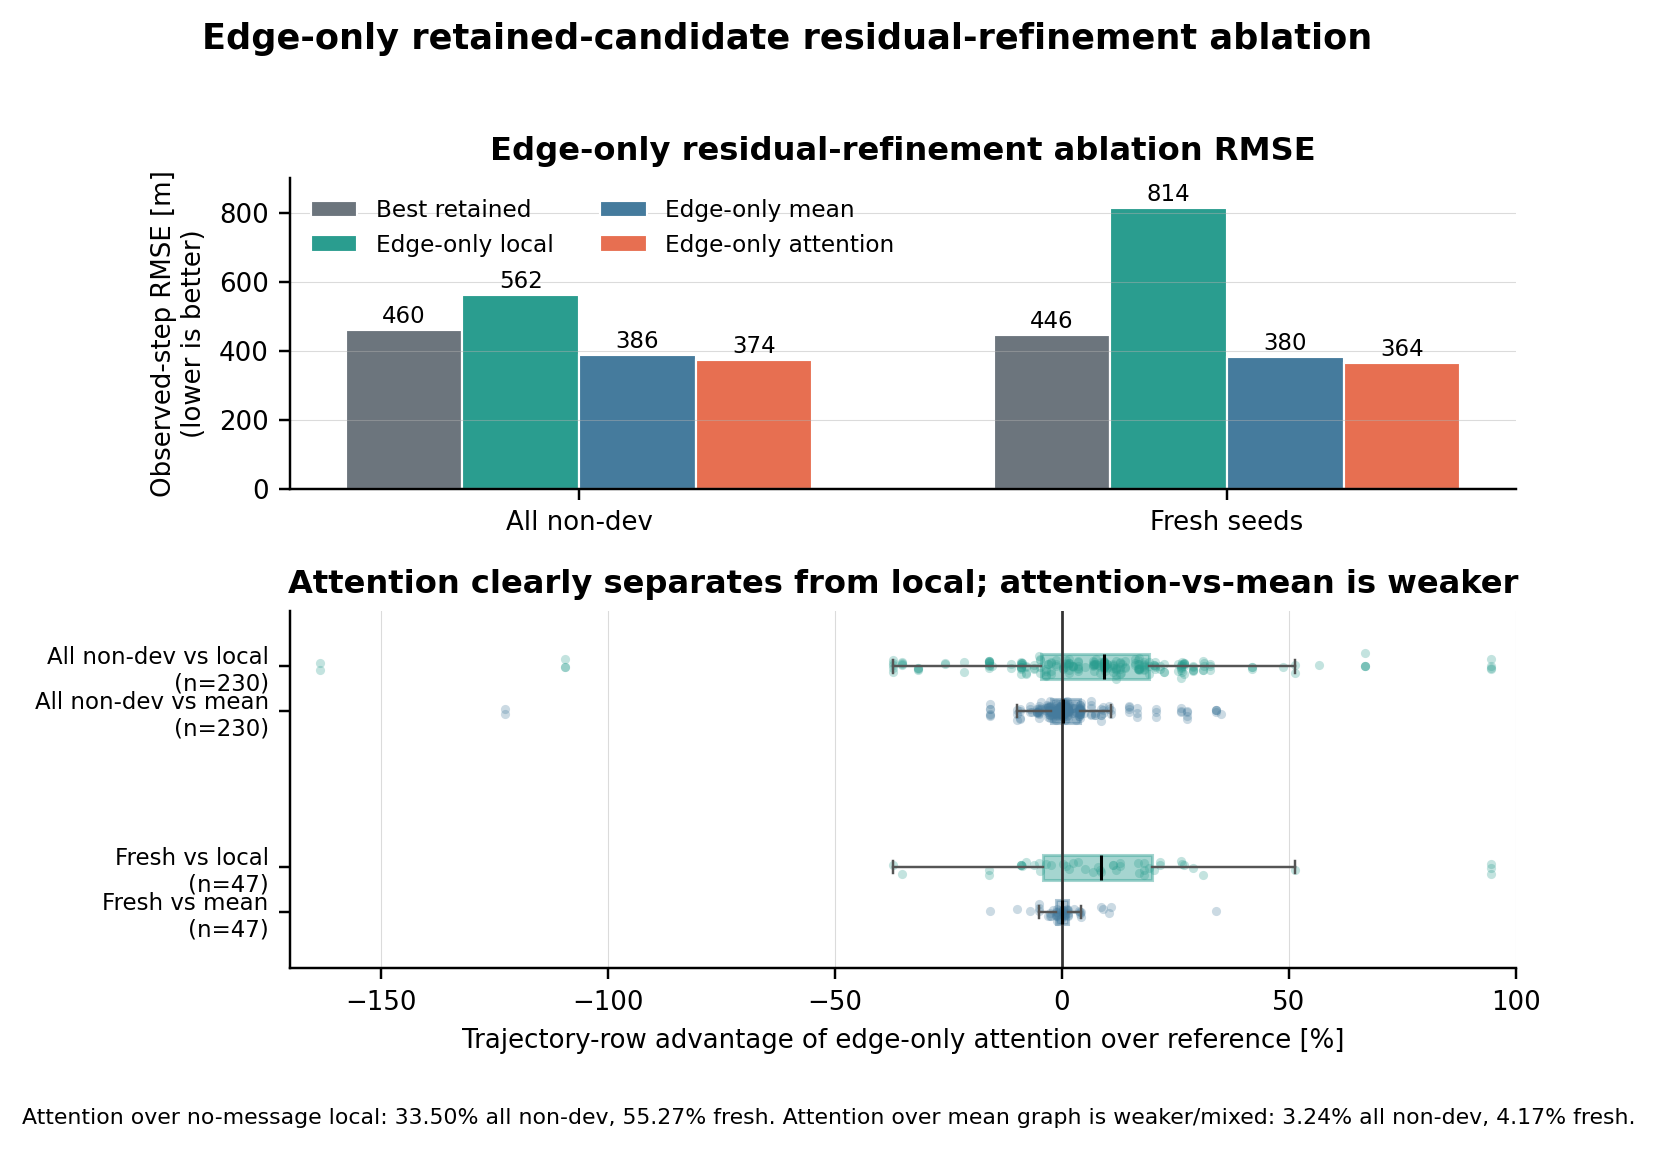
\includegraphics[width=\linewidth]{figures/trajectory_residual_refine_gain_distribution.png}
  \caption{Compact main-text view of the edge-only retained-candidate residual-refinement ablation, generated from row and summary artifacts in the edge-only attention, mean, and local residual-refinement directories. Lower observed-step RMSE is better. Omitting node-disagreement aggregates leaves graph layers with pairwise edge distance/overlap features only; within that setup, attention residual-refinement beats the matched no-message local control by 33.504\% on all non-development rows and 55.270\% on fresh unseen source-generation rows. The attention-vs-mean comparison is weaker/mixed: 3.235\% all non-development with the row CI crossing zero and 4.167\% fresh with intervals crossing zero. This is learned retained-candidate residual-refinement evidence only: graph-path isolation versus a matched no-message local control inside this compact retained-candidate ablation, not operational POD, not public precise-reference validation, not independent-machine reproduction, not a full raw/training/all-filter rerun, not standalone learned recursive filtering, not broad learned-OD validation, and not operational learned OD.}
  \label{fig:trajectory_residual_refine_gain_distribution}
\end{figure}

\begin{table*}[t]
\centering
\caption{Post-freeze retained-candidate learned-output proof of concept with the validation-selected edge-only residual-refinement ablation. The edge-only attention run uses member seeds 2111/2117/2129, \texttt{prediction\_mode=residual\_refine}, \texttt{residual\_loss\_weight=1e-5}, two attention graph layers, and \texttt{--node-disagreement-features omit}; this reduces the node feature dimension from 30 to 22 while leaving the 10 pairwise edge distance/overlap features available only to graph-message-passing layers. This validation-selected run used development validation seed minimum 53, 82 fit/training samples, 37 validation samples, and \texttt{validation\_loss} checkpoint selection. The matched edge-only local control has no message-passing layers, and the edge-only mean graph is a stronger graph comparator. The earlier train-loss edge-only run is historical exploratory evidence only because it used 119 fit/training samples, 0 validation samples, and train-loss checkpoint selection. The isolated claim is narrow: within this retained-candidate edge-only ablation, attention graph-path message passing cleanly beats the matched no-message local control, while attention-vs-mean evidence is smaller and the future-only attention-vs-mean check remains weak/mixed.}
\label{tab:main_trajectory_graph_selector_ensemble_poc}
\scriptsize
\setlength{\tabcolsep}{2.4pt}
\begin{tabular}{llrrrrrl}
\toprule
Aggregate & Comparison & Rows & Steps & Learned RMSE (m) & Baseline RMSE (m) & Gain (\%) & W/T/L and interpretation \\
\midrule
All non-development & Validation-selected edge-only attention residual-refine vs best-single & 230 & 6831 & 390.317 & 459.591 & 15.073 & 154/0/76; positive row/source-scenario gain CIs [11.451,18.575]/[11.739,18.307]\%. \\
All non-development & Validation-selected edge-only attention residual-refine vs local/no-message & 230 & 6831 & 390.317 & 519.282 & 24.835 & 150/0/80; positive graph-path/message-passing advantage over the matched no-message local control, CIs [11.172,36.097]/[12.108,35.630]\%. \\
All non-development & Validation-selected edge-only attention residual-refine vs mean graph & 230 & 6831 & 390.317 & 406.509 & 3.983 & 124/0/106; small positive advantage, CIs [1.522,6.654]/[1.563,6.385]\%. \\
Fresh extra seeds 151/157/163/167 & Validation-selected edge-only attention residual-refine vs best-single & 47 & 1426 & 386.373 & 445.943 & 13.358 & 29/0/18; positive row/source-scenario gain CIs [5.395,20.688]/[6.347,18.328]\%. \\
Fresh extra seeds 151/157/163/167 & Validation-selected edge-only attention residual-refine vs local/no-message & 47 & 1426 & 386.373 & 706.730 & 45.329 & 31/0/16; positive graph-path/message-passing advantage over local, CIs [6.233,61.137]/[23.030,59.308]\%. \\
Fresh extra seeds 151/157/163/167 & Validation-selected edge-only attention residual-refine vs mean graph & 47 & 1426 & 386.373 & 409.067 & 5.548 & 27/0/20; small positive advantage, CIs [0.441,11.744]/[0.774,11.825]\%. \\
Future-only subset & Validation-selected edge-only attention residual-refine vs mean graph & 136 & 4109 & 409.350 & 424.125 & 3.483 & Future-only attention-vs-mean check remains weak/mixed: row/source-scenario CIs [-0.296,8.590]/[-0.097,7.475]\%. \\
\bottomrule
\end{tabular}
\vspace{0.3em}
\scriptsize Sources: validation-selected edge-only attention residual-refinement records at \nolinkurl{results/trajectory_candidate_graph_attention_nodeomit_residual_refine_val53_ensemble3_2111_2117_2129_newfresh151157163167_20260625/summary.json}, \nolinkurl{results/trajectory_candidate_graph_attention_nodeomit_residual_refine_val53_ensemble3_2111_2117_2129_newfresh151157163167_20260625/rows.csv}, \nolinkurl{results/trajectory_candidate_graph_attention_nodeomit_residual_refine_val53_ensemble3_2111_2117_2129_newfresh151157163167_20260625/comparison_intervals.json}, and \nolinkurl{results/trajectory_candidate_graph_attention_nodeomit_residual_refine_val53_ensemble3_2111_2117_2129_newfresh151157163167_20260625/comparison_intervals.md}; validation-selected edge-only mean graph records at \nolinkurl{results/trajectory_candidate_mean_nodeomit_residual_refine_val53_ensemble3_2111_2117_2129_newfresh151157163167_20260625/summary.json} and \nolinkurl{results/trajectory_candidate_mean_nodeomit_residual_refine_val53_ensemble3_2111_2117_2129_newfresh151157163167_20260625/rows.csv}; validation-selected edge-only local/no-message records at \nolinkurl{results/trajectory_candidate_local_nodeomit_residual_refine_val53_ensemble3_2111_2117_2129_newfresh151157163167_20260625/summary.json} and \nolinkurl{results/trajectory_candidate_local_nodeomit_residual_refine_val53_ensemble3_2111_2117_2129_newfresh151157163167_20260625/rows.csv}; local tail diagnostic at \nolinkurl{results/trajectory_candidate_edge_only_local_tail_diagnostic_val53_20260625/summary.json}, \nolinkurl{results/trajectory_candidate_edge_only_local_tail_diagnostic_val53_20260625/summary.md}, and \nolinkurl{results/trajectory_candidate_edge_only_local_tail_diagnostic_val53_20260625/rows.csv}; figure at \nolinkurl{paper/figures/trajectory_residual_refine_gain_distribution_val53.png}; interval regeneration script \nolinkurl{scripts/build_trajectory_residual_refine_comparison_intervals.py}; tail diagnostic script \nolinkurl{scripts/build_trajectory_residual_refine_tail_diagnostic.py}. Eval truth scores rows and baselines only; residual-refinement training is simulator truth-supervised. This validation-selected edge-only run used development validation seed minimum 53, 82 fit/training samples, 37 validation samples, and \texttt{validation\_loss} checkpoint selection. The branch remains retained-candidate compact-simulator evidence only, not independent-machine reproduction, not operational POD validation, not public precise-reference validation, not a full raw/training/all-filter rerun, not standalone recursive filtering, not broad learned-OD validation, and not operational learned OD.
\end{table*}

\paragraph{Post-freeze row-weighted DLS side branch.}
A later compact-simulator PoC tests a learned row-weighted damped least-squares correction on \texttt{credible\_dense\_od\_test}. The graph row-WDLS model beats validation-selected fixed DLS on all five split seeds, with mean fixed-minus-learned RMSE delta 0.054797~m, mean gain 0.019178\%, and mean gain versus the best raw EKF/UKF candidate 0.582936\%. The no-message control is nearly equivalent: 5/5 wins versus fixed DLS, mean delta 0.052074~m, mean gain 0.018082\%, and mean gain versus best raw 0.581845\%. Graph beats no-message on only 3/5 seeds and the mean graph-vs-no-message advantage is only about 0.0027~m. Table~\ref{tab:main_row_weighted_dls_poc} therefore reports the PoC as a below-floor diagnostic side branch with no public precise-reference validation, no operational POD claim, no confirmatory learned-superiority claim, and no isolated message-passing contribution; retained artifact paths are listed in the supplement rather than in the Results prose.

\begin{table*}[t]
\centering
\caption{Post-freeze row-weighted damped least-squares (row-WDLS) compact-simulator proof of concept on \texttt{credible\_dense\_od\_test}. Positive gains mean lower observed-step position RMSE than the reference. The graph row-WDLS and no-message control both learn per-measurement-row weights inside the validation-selected DLS normal equations; their near-equivalence and below-floor gains make this a compact diagnostic side branch, not public precise-reference validation, learned-superiority validation, or an isolated graph/message-passing causal claim.}
\label{tab:main_row_weighted_dls_poc}
\scriptsize
\resizebox{\textwidth}{!}{%
\begin{tabular}{llrrrrrr}
\toprule
Seed & Variant & Learned RMSE (m) & Fixed DLS (m) & Best raw (m) & Gain vs fixed (\%) & Gain vs raw (\%) & Best epoch \\
\midrule
7 & Graph row-WDLS & 295.694 & 295.758 & 297.503 & 0.0216 & 0.608 & 1 \\
7 & No-message control & 295.685 & 295.758 & 297.503 & 0.0250 & 0.611 & 1 \\
11 & Graph row-WDLS & 291.429 & 291.512 & 292.713 & 0.0286 & 0.439 & 1 \\
11 & No-message control & 291.446 & 291.512 & 292.713 & 0.0227 & 0.433 & 1 \\
13 & Graph row-WDLS & 307.779 & 307.829 & 309.510 & 0.0163 & 0.559 & 6 \\
13 & No-message control & 307.771 & 307.829 & 309.510 & 0.0191 & 0.562 & 5 \\
17 & Graph row-WDLS & 264.922 & 264.954 & 267.113 & 0.0122 & 0.820 & 1 \\
17 & No-message control & 264.930 & 264.954 & 267.113 & 0.0094 & 0.817 & 1 \\
19 & Graph row-WDLS & 257.179 & 257.223 & 258.441 & 0.0172 & 0.488 & 1 \\
19 & No-message control & 257.187 & 257.223 & 258.441 & 0.0142 & 0.485 & 1 \\
\addlinespace
\multicolumn{8}{p{0.92\textwidth}}{Graph row-WDLS aggregate: 5/5 wins vs.\ fixed DLS; mean fixed-minus-learned RMSE delta 0.054797 m; mean, median, and minimum gains vs.\ fixed DLS 0.019178\%, 0.017163\%, and 0.012174\%; mean gain vs.\ best raw 0.582936\%.} \\
\multicolumn{8}{p{0.92\textwidth}}{No-message aggregate: 5/5 wins vs.\ fixed DLS; mean fixed-minus-learned RMSE delta 0.052074 m; mean, median, and minimum gains vs.\ fixed DLS 0.018082\%, 0.019116\%, and 0.009404\%; mean gain vs.\ best raw 0.581845\%. Graph beats no-message on 3/5 seeds, with only about 0.0027 m mean graph-vs-no-message advantage.} \\
\bottomrule
\end{tabular}%
}
\\[2pt]{\footnotesize The absolute gains over fixed DLS are centimetre-scale on a 257--308 m observed-step RMSE slice and well below the study's 3\% practical floor; the graph-vs-no-message comparison does not isolate message passing.}
\end{table*}


The $K=32$ frozen-rule replication has limited sensitivity to an exactly floor-sized stress effect (approximate power $\approx0.42$ at the 27.5~m floor under a one-sided $\alpha=0.05$ $t$-approximation; under the predicate's stricter two-sided 95\% CI rule the realized floor power is somewhat lower), so power is reported at the predeclared floor effect rather than at the realized gap; with the realized stress-row paired-gap variance, about $K\approx94$ independent realizations would be needed for roughly 0.80 power at that floor. The stress-only $K=96$ internal replication exceeds that design check for approximately 0.80 power at the 27.5~m floor and preserves the negative, but it remains internal, simulator-bound evidence under the already selected endpoint.

\section{Limitations and Missing Experiments}
Results are evaluation evidence for the documented simulation protocol, windows, baselines, and reported tables. They do not validate the estimator for flight operations, real-time integrated testbed deployment, safety-critical autonomy, or all sparse-visibility regimes. The EnKF boundary evidence comprises a canonical untuned stochastic EnKF check (S-Table~\ref{tab:enkf_comparator}) plus a validation-only inflation audit (S-Table~\ref{tab:validation_tuned_enkf_comparator}) that selected \(1.00\), no added inflation, after larger inflation values degraded validation performance; neither produces an EnKF positive on the frozen test slices. Localized EnKF variants, sequential Monte Carlo OD methods, ensemble-size search, and broader process-noise or covariance retuning remain outside this comparator set, so the bounded ensemble-Kalman negative should not be read as addressing the broader ensemble-filter design space. Likewise, cislunar particle/Gaussian-mixture filters and coupled orbit-attitude/sensor-tasking frameworks are cited as adjacent operational/filtering context, not as comparator baselines addressed by the tested claims. The residual-refinement comparisons are descriptive and branch-specific. In the original node-aggregate residual-refinement run, attention remains positive versus best retained candidates, but its graph-over-local residual intervals cross zero, so that result does not isolate message passing. In the new edge-only residual-refinement ablation, attention cleanly beats the matched edge-only no-message local control on all non-development and fresh aggregates, giving graph-path isolation only within that matched local-control contrast. Attention-vs-mean graph evidence is weaker/mixed, so causal or architectural interpretation remains bounded. The branch still requires independent/full rerun and public precise-reference validation before broader or operational interpretation; it also depends on retained candidate trajectories and simulator truth-supervised training, so it is not a standalone recursive filter or operational learned OD. The auxiliary replay, controlled-synthetic, and bounded public precise-reference slices are stress/provenance probes rather than operational OD.

The worked inspection record is a self-evaluation: the record is designed by the authors and applied primarily to the authors' own residual constructions, plus in-house learned-gain and adapted-transposition probes. That structure can falsify the authors' own claims before escalation, but it is not independent third-party validation of a reusable framework and does not show that another group would instantiate the same seven ingredients or reach the same boundaries. The visible-record positioning definitions are self-authored operational definitions, which makes them inspection boundaries rather than an externally ratified novelty taxonomy. This negative is architecture-family specific to the tested constructions and compact sparse-visibility setting. The present contribution is a worked, inspectable compact-simulator audit record; independent application by a separate research group is the next evidentiary tier before any generally validated reusable-framework claim.

The post-hoc endpoint-timeline concern qualifies the primary endpoint ranking evidence; it does not drive the AUKF \(R\)-inflation or drag-scale cascade mechanism findings, and the DBAR withdrawal follows its own characterization rather than learned endpoint selection. The designated next step for this specific limitation is an externally timestamped digest of a prospective decision rule, committed before and bound to an independent public precise-reference replication carried out by a separate party, with no rule content disclosed at timestamping; this is future work, neither completed here nor claimed as external trial-registry preregistration.

The public LAGEOS/SP3 compact-filter readout is only a bounded real-measurement adaptive-filter transfer diagnostic for the DBAR/AUKF \(R\)-inflation warning: the statistic is computed from the real AUKF-versus-fixed-UKF innovation and \(R\)-adaptation stream, while the outcome label is defined externally from held-out SP3 state error, not from the DBAR statistic and not from a simulator label (S-Tables~\ref{tab:real_slr_sp3_od} and~\ref{tab:real_slr_sp3_od_expanded}). The original ten-arc slice, extended 80-arc replay, and formal 210-arc replay remain archival evidence; the formal 400-arc replay supersedes the earlier campaigns as the strongest compact real-data diagnostic. It attempted 400 arcs; 373 completed; the 27 non-completed arcs are explicit status records in the validation records (17 insufficient observations; 10 public product unavailable or non-parseable), not hidden or imputed. The completed count clears the earlier approximate 185 comparable-arc formal power target (comparable arc: completed arc with at least 10 CRD normal points and SP3 state coverage), but the result remains negative. DBAR is correct on 256/373 arcs (0.686), below the 0.737 always-``no-fire'' majority baseline, with sensitivity 0.480 and specificity 0.760; EKF-minus-AUKF mean $-34.78$~m has median $-0.76$~m and 95\% CI $[-71.84,-2.76]$~m, and fixed-noise-UKF-minus-AUKF mean $-28.14$~m has median $-0.77$~m and CI $[-61.80,-2.75]$~m. Under the first-minus-second convention, those strictly negative intervals mean AUKF has larger held-out RMSE on average than EKF and fixed-noise UKF. The supplementary completed-only stratification shows non-stable ordering across preceding/train/validation/test splits and across LAGEOS-1/LAGEOS-2; the wider formal 400-arc intervals are therefore best treated as epoch, target, arc-geometry, and unmodelled perturbation/frame-reduction heterogeneity rather than stable filter superiority, with no causal attribution. The larger replay therefore supports withdrawing DBAR and treating the compact-model \(R\)-inflation mechanism as a hypothesis for future real-data studies; it does not validate the simulator conclusion, establish operational POD, or provide real-data learned estimator-skill evidence.

The simulator omits several failure modes that bound interpretation of the negative results. It does not include maneuvers, thrust events, attitude-coupled force errors, clock-estimation states, sensor timing biases, heterogeneous station instrumentation, decoded RF observables, onboard GNSS ambiguity handling, or a multi-class operational tracking network. Its estimator-side dynamics deliberately stay below an operational force-model ceiling; the long-arc and public probes test selected pressure points, not the full space of high-fidelity force, sensor, and reference-model errors. Consequently, a negative in this paper weighs against advancing the tested claims within the documented sparse-visibility setting, but it does not transfer as a negative about a different sensor geometry, mission class, or operational POD system.

The compact-physics ceiling is also a mechanism limitation. A learned above-floor positive requires residuals that are jointly \emph{observable} from the visible measurements and \emph{representable} by the candidate relative to the prior/filter bank. Each originally audited negative fails at least one gate: on the noise-side stress split the signal is already represented by AUKF, while on the force-side mismatch and drag-scale cascade it is unobservable from sparse line-of-sight geometry and/or unrepresentable by the compact prior. The post-freeze row-weighted DLS PoC is a different anchored correction family and records only below-floor centimetre-scale gains over fixed DLS on one credible-dense slice. This is descriptive of the tested constructions, not a general impossibility result. Offline WLS, multi-revolution public-catalog, and public precise-reference probes show that compact dynamics and sparse geometry dominate large parts of the residual budget, so the result is a pre-campaign evidence-triage negative for the tested constructions under this compact prior, not a claim that learned correction could never help under a different force model, sensor, or public-reference regime.

Before operational deployment, future validation must bridge from compact-sim gates (learned candidates surpass tuned adaptive guardrails, frozen endpoints, practical floors, structural channels) to higher-fidelity simulation, real held-out arcs with independent precise reference, and operations-facing metrics. A focused falsification test would precommit the fixed AUKF \(R\)-inflation rule and ask whether it predicts held-out real-error degradation on independent precise-reference or higher-fidelity arcs; failure would confine the mechanism to the compact simulator, while success would only justify further real-data validation rather than establish operational POD. This study covers only compact-sim gates, and the long-arc EKF/AUKF reversal shows compact-AUKF prescription is regime-bound.

Missing experiments are concrete: centimetre-level precise SLR reduction; real high-fidelity force-error campaigns; maneuvers; powered, independently sized reference-state scoring of learned estimators on real measurements beyond the bounded public probes; decoded RF measurements; independent external confirmation or operational validation of the endpoint result; and faithful reproduction of specific published learned-OD systems in their own documented settings. Highest-priority follow-ups are topology generalization to held-out satellites, stations, and geometries; high-fidelity force/sensor mismatch beyond the current controlled split; held-out public-campaign generalization for any learned candidate advanced beyond screening; broader non-graph parameter-matched ablations with public precise-reference validation; and independent public precise-reference validation beyond replay-style evidence.

\paragraph{Public replay scope and deployment boundary.}
The robustness claims are limited to the synthetic measurement, visibility, and noise regimes summarized in the reported tables and figures. Under the time-aligned SatNOGS observation-window replay (Appendix~\ref{app:supplementary}) the EKF stays finite at kilometre scale and offline robust batch WLS produces an accurate postfit OD solution, so that slice is a bounded classical/offline-OD validation, not a universal-failure slice or confirmatory deployment evidence \cite{satnogs_network}.

\section{Data and Reproducibility Statement}
\label{sec:data-reproducibility}

The evaluation suite uses archived inputs, fixed random seeds, documented simulator settings, and reported result tables. Archived CelesTrak and SatNOGS snapshots replace live API queries, so replay scenarios are not affected by later public-service changes. Public precise-reference probes use real ILRS satellite-laser-ranging normal points for LAGEOS-1 and LAGEOS-2 together with independent ILRS NSGF SP3-c products; consistent with Section~\ref{sec:claim-audit}, they are provenance and measurement-pipeline evidence under the claim hierarchy, not operational POD or real-data learned-estimator validation. Synthetic nominal and stress splits use fixed orbit, force-model, visibility, and measurement-noise settings, and all methods are evaluated over a common scoring horizon.

Without confidential journal-review materials, a public reader can inspect the coherent public GitHub release archives, verify the released archive identifiers and hashes where the archive is obtained, inspect manifest and generated-artifact records exposed in the release family, and rerun the packaged archived-input public CRD/SP3 slice described in Data availability. Public materials also expose the source and diagnostic summaries for the original v1.2.7 retained-candidate residual-refinement PoC and the packaged GraphAnchorPairGate and AdaptiveCandidateFusion side branches; the published v1.2.8 archive/metadata/figure clarification release now supersedes the earlier metadata-inconsistent v1.2.7 Zenodo import. The edge-only residual-refinement ablation is documented through local row/summary artifacts and the regeneration scripts cited in Table~\ref{tab:main_trajectory_graph_selector_ensemble_poc}. These materials do not expose the confidential retained digests, complete selected lower-priority numeric records, trained-estimator/evaluation records, or inspection-material extraction checks, and they do not provide full raw/training/all-filter public reproduction, full seed-suite regeneration, independent-machine confirmation, live public-data retrieval, or operational precise-reference reproduction.

The versioned supplementary evidence package records the fixed data settings, input and output digests, predeclared rules, seeds, splits, selected models, validation criteria, and evaluation records used by the reported tables. The inspection materials contain the evidence file and manifest; the supplement quotes the primary endpoint, $K=32$ frozen-rule, and stress-only $K=96$ rule records so that the core predeclaration language is visible in the manuscript package. Logged checks cover compiled-package readback, archive-extracted public-slice rerun, minimum-tier manifest/digest audit, active-regeneration checks for the main-manuscript generated inputs, and one bounded learned-estimator replay. The post-freeze GraphAnchorPairGate, AdaptiveCandidateFusion, trajectory candidate selector, and row-weighted DLS records are retained as compact-simulator diagnostics rather than operational or independent-reproduction evidence. The archive-extracted rerun recomputes the range-only filters from recorded public CRD/SP3 inputs, reproduces the submitted table text exactly, and matches the recorded public claim summary with zero field mismatches. These checks strengthen inspection and rerun readiness below full scientific reproduction; Data availability states the public access and scope boundary.

Archive membership, manifest coverage, and SHA-256 digest checks establish submitted-package integrity and claim-map coverage; they do not constitute full scientific reproduction. The current package includes bounded all-filter readbacks, live public-week scoring artifacts, and one non-destructive single rerun at \nolinkurl{results/full_rerun_20260616}: status pass, completed on 2026-06-17T13:57:27+02:00, regenerated raw data, trained the enabled learned models, and evaluated the classical and learned methods across the scenario set without overwriting submitted canonical artifacts. That rerun is evidence of internal rerun reach only. It is not full multi-seed learned-estimator retraining, independent-machine confirmation, operational precise-reference reproduction, or a clean replacement of submitted manuscript tables or figures. It also exposed divergence flags on \texttt{dense\_visibility\_test} and \texttt{satnogs\_observation\_replay\_test}, including UKF/AUKF and several learned residual families; the divergence audit at \nolinkurl{results/validation/full_rerun_divergence_audit_20260617.md} treats all failure-conditioned summaries as diagnostic only, not replacements for canonical decision metrics or practical-floor logic. The post-freeze portfolio records remain archived reproduction-support diagnostics in the supplement and cited release boundaries; they are not full scientific reproduction, active main-text evidence, or endpoint replacements.

One bounded learned-estimator training replay runs the full materialized curriculum shape on deterministic retained slices: 160 nominal training, 32 nominal validation, 96 stress-training, 24 stress-validation, and 16 SatNOGS replay-validation trajectories. It records finite stage histories, checkpoint and manifest digests, and an unchanged canonical checkpoint digest while leaving the submitted trained-estimator records unchanged. In parallel, the official KalmanNet release is rerun end-to-end on its native linear-canonical benchmark inside the evidence package and recovers the expected ordering observation-floor $>$ KalmanNet $\geq$ optimal KF, with KalmanNet test error within 2~dB of the optimal KF on that upstream benchmark. These remain bounded inspection artifacts; a stronger scientific reproduction tier would require independent-machine replay, multi-seed repetitions, full raw/training/all-filter regeneration, and reconciliation of divergence-flagged stress slices.

\section{Conclusion}
The primary finding is a compact-simulator AUKF R-inflation diagnostic: under force-model mismatch in a compact two-body+$J_2$+drag OD simulator, AUKF inflates effective \(R\) (mean 3.32; median \(R\)-only NIS 4.73 versus 1.60/1.83 for EKF/UKF) and damps needed state corrections, quantifying an OD-specific instance of the known covariance-matching failure mode. The drag-scale cascade separates EKF linearisation, sparse-geometry observability, and candidate-inertia limits as distinct binding constraints. The mechanism result is reproduced in the controlled diagnostic and is further supported by the R-inflation cap control (S-Table~\ref{tab:constrained_aukf_mechanism_control}); the sampled true-pre-update innovation campaign preserves a high-specificity/low-recall warning boundary inside the compact sampled frame, while the higher-fidelity pre-update repeat and the supplement's long-arc EKF/AUKF stress observation confine that warning to its tested regime. These compact-simulator findings (350--925~m scale) require precise-reference validation before operational transfer; the indeterminate 260606 public-week readout, usable EDC 260613 SP3 products, unavailable/placeholder 260620 and 260627 products, and CDDIS login/HTML status reduce provenance ambiguity but do not close that validation gap. Operational ILRS/SP3 analyses operate at centimetre/sub-metre accuracy under higher-fidelity reductions, a scale not addressed here.

The learned-estimator record is secondary to that mechanism result. For the originally audited residual/GNN/KalmanNet-style family, the primary observed-step endpoint and the internal $K=32$/$K=96$ frozen-rule replications find no learned construction that beats the per-scenario best tuned classical reference; endpoint-choice, structural-channel, DBAR, EnKF, and KalmanNet-transposition diagnostics do not upgrade that result into a broad learned-OD claim. The post-freeze retained-candidate learned-output branch is the first material learned-method PoC in this evidence package and is positive on retained non-development and fresh unseen source-seed aggregates. Its strongest current variant is the edge-only attention graph residual-refinement ensemble, which outputs a probability-weighted retained-candidate trajectory plus learned constant 3D per-candidate offsets and supersedes the released pure attention selector. Omitting node-disagreement aggregates creates a narrow graph-path isolation test: attention cleanly beats the matched no-message local control, while attention-vs-mean is weaker/mixed. The original node-aggregate residual-refine variant remains positive versus best retained, but its graph-over-local intervals cross zero. The branch still depends on retained candidate trajectories and simulator truth-supervised training, is not a standalone learned recursive filter, and has no public precise-reference, independent-machine, full raw/training/all-filter rerun, operational POD, operational learned OD, or broad learned-OD validation. Post-freeze GraphAnchorPairGate, AdaptiveCandidateFusion, and row-weighted DLS remain compact-simulator side branches below the primary endpoint. The row-weighted DLS graph PoC beats fixed DLS on five credible-dense splits, but with small absolute gains, no public precise-reference validation, and no isolated message-passing contribution. The learned-side record is therefore bounded to the tested constructions: it is not confirmatory learned-superiority evidence, operational POD evidence, or a universal learned-OD result.

The empirical contribution is the compact AUKF \(R\)-inflation and drag-scale observability mechanism; the supporting materials provide an inspection/reproducibility scaffold for this study. The manuscript should therefore be read as a compact-audit note on one simulator-bound mechanism and its evidence boundary, not as a full operational validation or reusable framework paper. Other OD regimes would need their own endpoint hierarchy, frozen decision rules, classical and offline guardrails, capacity-matched controls, practical floors, evidence records, datasets, baselines, and external-reference checks. Independent external application is the next evidentiary tier before any reusable-framework claim.

\paragraph{Campaign-planning workflow.}
For small-satellite teams screening learned candidates, the worked compact-simulator gate is: beat the per-scenario best tuned adaptive guardrail on observed-step RMSE by the practical floor, survive paired-bootstrap CIs and frozen K=32-scale rules, move a structural drag-scale channel under sparse visibility, avoid provenance false-positive triggers, and then escalate to precise-reference validation. In this record, RGR-GF and the structural channels fail: RGR-GF loses to AUKF on stress (gap +31.9 m after powered K=96) and to EKF on force-mismatch (gap +16.8 m after K=32), DSA-EKF remains below practical floor, and DBAR withdraws after 450-realization characterization. Within this compact screening regime, AUKF remains the adaptive guardrail to beat before higher-fidelity campaign work. Confirmatory use still requires prospectively fixed external validation.

\section{Reproduction checklist}\label{sec:repro-checklist}
Every headline maps to supplementary evidence materials. The logged checks cover compiled-PDF readback, citations, release-packet synchronization, zero-warning LaTeX logs, current-workspace active manuscript regeneration for the main generated inputs, archive-extracted public-slice rerun from recorded CRD/SP3 inputs, minimum-tier manifest/digest coverage, bounded learned-estimator and KalmanNet replays, EnKF/readback checks, compact and higher-fidelity true-pre-update AUKF/UKF sampled innovation campaigns, live 260606 public-week scoring, and \texttt{results/full\_rerun\_20260616}. These are inspection checks below full scientific reproduction, not operational POD validation. The edge-only attention graph residual-refinement ensemble is the strongest current retained-candidate learned-output PoC, while the released pure attention selector, GraphAnchorPairGate, AdaptiveCandidateFusion, and row-weighted DLS records stay below confirmatory learned-superiority evidence. Its graph-path isolation is limited to the matched edge-only no-message local control; attention-vs-mean is weaker/mixed, and the original node-aggregate residual-refine graph-over-local intervals cross zero. Independent/full rerun and public precise-reference validation therefore remain deeper evidence tiers before causal/operational interpretation. The coherent public GitHub release for the original v1.2.7 residual-refinement evidence is \nolinkurl{https://github.com/Alavi1412/spot-od-reproduction/releases/tag/v1.2.7-residual-refine-poc}. The archive/metadata/figure clarification release is now published as \texttt{v1.2.8-residual-refine-figure-archive-fix}: GitHub release \nolinkurl{https://github.com/Alavi1412/spot-od-reproduction/releases/tag/v1.2.8-residual-refine-figure-archive-fix}, target commit \texttt{6ca71ff41f4270e6ce6022e1c5fd94b8fe44ebcf}, release asset \nolinkurl{spot_od_v1_2_8_residual_refine_figure_archive_fix.zip} (5,230,470 bytes; SHA-256 \texttt{3FE91FAA780E446728B430972146FEEC4A12F115182C048FFF1377B71F4D6ACB}), Zenodo record \nolinkurl{https://zenodo.org/records/20840386}, DOI \nolinkurl{10.5281/zenodo.20840386}, and concept DOI \nolinkurl{10.5281/zenodo.20768672}. The earlier \nolinkurl{10.5281/zenodo.20839901} record is the superseded metadata-inconsistent v1.2.7 import: visible metadata retained stale v1.2.5 text while the file was v1.2.7, so it is not current or latest evidence. v1.2.8 is an archive/metadata/figure clarification only and adds no new scientific validation: it is not operational POD, not public precise-reference validation, not independent-machine reproduction, not a full raw/training/all-filter rerun, not standalone learned recursive filtering, not broad learned-OD validation, and not operational learned OD. The full rerun is not a new manuscript-table source and remains caveated by divergence flags on dense-visibility and SatNOGS replay slices; public slices remain measurement-pipeline/provenance checks rather than operational POD validation. Full multi-seed learned-estimator training, full seed-suite regeneration, full raw/training/all-filter public reproduction, live public-data retrieval, independent-machine confirmation, and operational precise-reference reproduction remain deeper evidence tiers. Data availability defines the public release scope and the remaining confidential/full-rerun boundaries.

Each headline therefore points to recorded input-data digests, predeclared rule records, and records that fix seeds, splits, trained models, and selection rules. The access mechanisms and scope boundaries are stated once in Data availability; this checklist maps claims to the records needed for inspection or deeper reruns.

\section*{Supplementary material}
\label{sec:supplementary-material-pointer}
The complete learned-estimator architecture and training-objective specification, the bounding and diagnostic tables that support but are not central to the claim-audited negative, and the four temporal/calibration figures are reported in the separate supplementary document that accompanies this manuscript. The supplement provides full printed table bodies for core and boundary material (the multiplicity-adjusted family, the DBAR three-regime exhibition and 450-realization characterization, the densified-visibility control, and the matched-budget and SatNOGS-selection sensitivity tables); selected lower-priority archival records (precise-reference measurement-pipeline tables plus propagation/offline-OD/replay reference tables) appear as concise indexed summaries in the supplement, with their full numeric records supplied in the confidential journal-review evidence package. Cross-references from the main text to supplement-housed tables and figures use the S-Table/S-Figure prefix and resolve through the supplement's external label list.

\section*{Declaration of competing interest}
The authors declare no known competing financial interests or personal relationships that could have appeared to influence the work reported in this paper.

\section*{Funding}
This research did not receive any specific grant from funding agencies in the public, commercial, or not-for-profit sectors.

\section*{Data availability}
The confidential journal-submission package includes versioned dependency and evaluation records sufficient for inspection of the reported retained results. It covers fixed data settings, internally timestamped predeclared rule and seed records, trained-estimator records, evaluation records, learned-estimator specification records, recorded public input identifiers, and retained digest values used in the study. The main manuscript and supplement expose the claim hierarchy, table bodies or indexed summaries, rule excerpts, and key numeric results; the confidential package is needed to inspect retained digests, full selected lower-priority numeric records, trained-estimator/evaluation records, and inspection-material extraction checks.

A public archival reproduction-support repository is maintained at \nolinkurl{https://github.com/Alavi1412/spot-od-reproduction}. The coherent public GitHub release for the original retained-candidate residual-refinement evidence is \texttt{v1.2.7-residual-refine-poc}, \nolinkurl{https://github.com/Alavi1412/spot-od-reproduction/releases/tag/v1.2.7-residual-refine-poc}. The published archive/metadata/figure clarification release is \texttt{v1.2.8-residual-refine-figure-archive-fix}, \nolinkurl{https://github.com/Alavi1412/spot-od-reproduction/releases/tag/v1.2.8-residual-refine-figure-archive-fix}, target commit \texttt{6ca71ff41f4270e6ce6022e1c5fd94b8fe44ebcf}, with release asset \nolinkurl{spot_od_v1_2_8_residual_refine_figure_archive_fix.zip} (5,230,470 bytes; SHA-256 \texttt{3FE91FAA780E446728B430972146FEEC4A12F115182C048FFF1377B71F4D6ACB}) and clean Zenodo record \nolinkurl{https://zenodo.org/records/20840386}, DOI \nolinkurl{10.5281/zenodo.20840386}, concept DOI \nolinkurl{10.5281/zenodo.20768672}. The local evidence paths for the edge-only main-text residual-refinement ablation are \nolinkurl{results/trajectory_candidate_graph_attention_nodeomit_residual_refine_ensemble3_2111_2117_2129_newfresh151157163167_20260625/}, \nolinkurl{results/trajectory_candidate_mean_nodeomit_residual_refine_ensemble3_2111_2117_2129_newfresh151157163167_20260625/}, and \nolinkurl{results/trajectory_candidate_local_nodeomit_residual_refine_ensemble3_2111_2117_2129_newfresh151157163167_20260625/}; the compact figure is regenerated from their \texttt{rows.csv} and \texttt{summary.json} artifacts, and the interval file is regenerated by \nolinkurl{scripts/build_trajectory_residual_refine_comparison_intervals.py}. Earlier public releases such as \texttt{v1.2.3-acf-holdout-audit} and \texttt{v1.2.5-zenodo-metadata-repair} remain historical packaging and metadata-repair records, not the current residual-refinement evidence boundary.

The earlier \nolinkurl{10.5281/zenodo.20839901} record is the superseded metadata-inconsistent v1.2.7 import: the title/version metadata remained stale \texttt{v1.2.5} text while the archived file was v1.2.7. This mismatch is disclosed as historical release-metadata evidence only, not as the current clean public DOI record. The published v1.2.8 release preserves the same bounded evidence scope and only clarifies archive metadata and the residual-refinement figure/package status; it adds no new scientific validation and is not operational POD, not public precise-reference validation, not independent-machine reproduction, not a full raw/training/all-filter rerun, not standalone learned recursive filtering, not broad learned-OD validation, and not operational learned OD. The new edge-only graph-path isolation claim is local to the retained-candidate compact-simulator ablation versus a matched no-message local control.

The public release family is bounded reproduction-support evidence: archive extraction, manifest hashes, active manuscript artifact regeneration, one archived-input public OD slice rerun, and archived packaging of compact-simulator diagnostic/source artifacts. The submitted evidence also demonstrates internal record checks, generated-table consistency before and after inspection-material extraction, one public precise-reference OD slice-level rerun from submitted inspection materials, one bounded learned-estimator training replay, one official KalmanNet native-benchmark rerun, bounded EnKF comparator/audit records including a validation-only inflation audit that selected \(1.00\), no added inflation, cache-busted all-filter readbacks, one live public-week scoring pass, and one non-destructive single rerun under \nolinkurl{results/full_rerun_20260616}. That rerun is retained as diagnostic/reproducibility evidence only: it regenerated raw data, trained enabled learned models, and evaluated the classical and learned methods across the scenario set without overwriting submitted canonical artifacts, but it is not a generated-table replacement, independent-machine or full scientific reproduction, full raw/training/all-filter public reproduction, live public-data retrieval, operational POD validation, or third-party independent validation, and it exposed divergence flags on dense-visibility and SatNOGS replay slices. The retained-candidate residual-refinement, released pure selector, portfolio, and row-weighted DLS probes remain compact-simulator diagnostics below operational validation and below independent scientific reproduction; the edge-only attention graph residual-refinement ensemble is the strongest current retained-candidate learned-output PoC and isolates graph-path benefit only against its matched no-message local control, while attention-vs-mean is weaker/mixed. These checks strengthen inspection readiness; full multi-seed estimator retraining, independent-machine confirmation, full raw/training/all-filter regeneration, and operational precise-reference reproduction remain deeper rerun routes beyond the present release package.

\section*{Declaration of Generative AI and AI-assisted technologies in the writing process}
During the preparation of this manuscript, the authors used AI-assisted technologies to support prose organization, clarity revision, and consistency verification across the manuscript and supplementary materials. After using these tools, the authors reviewed and edited all content and take full responsibility for the scientific claims, evidence interpretation, and published content.

\bibliographystyle{plain}
\bibliography{references}

\end{document}
